\documentclass[a4paper,12pt]{amsart}
\input epsf
\usepackage{epsfig}
\usepackage{amsmath}
\usepackage{subcaption}

\DeclareMathAlphabet\mathbold{OML}{cmm}{b}{it}
\textheight=8.75in
\textwidth=6in
\oddsidemargin=-0.1in
\evensidemargin=-0.1in
\vsize 8.2in
% Equation numbering
\numberwithin{equation}{section}
 
\newtheorem{theorem}{Theorem}[section]
\newtheorem{lemma}{Lemma}[section]
\newtheorem{remark}{Remark}[section]
\newtheorem{corollary}{Corollary}[section]
\newtheorem{definition}{Definition}[section]
\newtheorem{algorithm}{Algorithm}[section]
\newtheorem{assumption}{Assumption}[section]
\newtheorem{example}{Example}[section]
\newtheorem{proposition}{Proposition}[section]





\newcommand{\curl}{\operatorname{curl}}
\renewcommand{\div}{\operatorname{div}}
\newcommand{\Div}{\operatorname{Div}}
\newcommand{\trace}{\operatorname{tr}}
\newcommand{\diag}{\operatorname{diag}}


\def\b1{{\mathbf 1}}
\def\bv{{\mathbf v}}
\def\bu{{\mathbf a}} % redefined
\def\bw{{\mathbf w}}
\def\bb{{\mathbf b}}
\def\bc{{\mathbf c}}
\def\bff{{\mathbf f}}
\def\bg{{\mathbf g}}
\def\bh{{\mathbf h}}
\def\br{{\mathbf r}}
\def\bs{{\mathbf s}}
\def\bd{{\mathbf d}}
\def\be{{\mathbf e}}
\def\bp{{\mathbf p}}
\def\bq{{\mathbf q}}
\def\bx{{\mathbf x}}
\def\by{{\mathbf y}}
\def\bz{{\mathbf z}}
\def\bn{{\mathbf n}}
\def\bbf{{\mathbf f}}
\def\bB{{\mathbf B}}
\def\bM{{\mathbf M}}
\def\bV{{\mathbf V}}
\def\bU{{\mathbf U}}
\def\bY{{\mathbf Y}}
\def\bF{{\mathbf F}}
\def\bA{{\mathbf A}}
\def\bB{{\mathbf B}}
\def\bC{{\mathbf C}}
\def\bD{{\mathbf D}}
\def\bN{{\mathbf N}}
\def\bT{{\mathbf T}}
\def\bP{{\mathbf P}}
\def\bQ{{\mathbf Q}}
\def\bS{{\mathbf S}}
\def\bR{{\mathbf R}}
 
\def\bepsilon{{\boldsymbol \epsilon}}
\def\balpha{{\boldsymbol \alpha}}
\def\bdelta{{\boldsymbol \delta}}
\def\blambda{{\boldsymbol \lambda}}
\def\bmu{{\boldsymbol \mu}}
 
 
 
%-----------------------------------------------------------------
\renewcommand{\O}{{\mathcal O}}
\newcommand{\Q}{{\mathcal Q}}
\newcommand{\R}{{\mathcal R}}
\newcommand{\A}{{\mathcal A}}
\newcommand{\B}{{\mathcal B}}
\newcommand{\C}{{\mathcal C}}
\newcommand{\D}{{\mathcal D}}
\newcommand{\Sc}{{\mathcal S}}
\newcommand{\F}{{\mathcal F}}
\newcommand{\G}{{\mathcal G}}
\newcommand{\I}{{\mathcal I}}
\newcommand{\J}{{\mathcal J}}
\newcommand{\M}{{\mathcal M}}
\newcommand{\N}{{\mathcal N}}
\newcommand{\X}{{\mathcal X}}
\newcommand{\Y}{{\mathcal Y}}
\newcommand{\calY}{{\mathcal Y}}
\newcommand{\calS}{{\mathcal S}}
\renewcommand{\L}{{\mathcal L}}
\renewcommand{\P}{{\mathcal P}}
 
\newcommand{\vertiii}[1]{{\left\vert\kern-0.25ex\left\vert\kern-0.25ex\left\vert #1 
    \right\vert\kern-0.25ex\right\vert\kern-0.25ex\right\vert}}
 
\newcommand{\V}{\text{\bf V}}
\newcommand{\K}{{\mathcal K}}
\newcommand{\T}{{\mathcal T}}
\newcommand{\E}{{\mathcal E}}

\newcommand{\hatcalK}{\widehat{\mathcal K}}
\newcommand{\hatcalS}{\widehat{\mathcal S}}
\newcommand{\hatA}{\widehat{A}}
%% \newcommand{\grad}{\nabla}
%% \renewcommand{\div}{\text{div}}
%% \renewcommand{\curl}{\text{curl}}
%
%
\def\XVec#1{{\mathbf #1}}
\def\XNorm#1{\left\| #1 \right\|}                       % norm
\def\XIProd#1#2{\left\langle #1 ,~ #2 \right\rangle}    % inner product
 
\def\XM{\mu}
 
\def\XQ{Q}                     % interpolant
\def\Xq#1{\XVec{q}_{#1}}       % rows of Q (interpolation to point #1)
\def\Xu{\XVec{u}}              % unknown vector
\def\Xf{\XVec{f}}              % right-hand-side vector
\def\Xe{\XVec{e}}
\def\Xr{\XVec{r}}
\def\Xx{\XVec{x}}
\def\Xv{\XVec{v}}
\def\Xw{\XVec{w}}
\def\Xn{\XVec{n}}              % normal vector
\def\Xes{\Xe_s}
\def\Xec{\Xe_c}
\def\Xus{\Xu_s}
\def\Xuc{\Xu_c}
\def\Xvs{\Xv_s}
\def\Xvc{\Xv_c}
\def\bone{{\boldsymbol 1}}
\def\bphi{{\boldsymbol \varphi}}
\def\bpsi{{\boldsymbol \psi}}
\def\bPsi{{\boldsymbol \Psi}}
\def\btheta{{\boldsymbol \theta}}
\def\bchi{{\boldsymbol \chi}}
\def\boldeta{{\boldsymbol \eta}}
\def\bolddelta{{\boldsymbol \delta}}
\def\bsigma{{\boldsymbol \sigma}}
\def\btau{{\boldsymbol \tau }}
\def\bxi{{\boldsymbol \xi }}
\def\bdelta{{\boldsymbol \delta}}
 
\def\Nedelec{N\'ed\'elec\ }

\def\bPi{{\boldsymbol \Pi}}
\def\bPhi{{\boldsymbol \Phi}}

\newcommand{\ott}[1]{\bar{#1}}
 

\newcommand{\dt}{\partial_t} 
\newcommand{\om}{\Omega} 

\renewcommand{\arraystretch}{1.2}

\DeclareMathOperator*{\argmin}{argmin}
 
 
\title[A minimization solver for AMR in CFOSLS, report] 
{A minimization solver for AMR in constrained first-order system least-squares, report}

\address{Portland State University}

\keywords{CFOSLS, space-time, adaptive mesh refinement, multilevel algorithms, multigrid}

\begin{document}
 
\begin{abstract}
Adaptive mesh refinement is studied for constrained first-order system least-squares (CFOSLS) formulations of linear transport (in space-time setting) and Laplace equations in 3D. The problems are considered as minimization problems, for which we use local functional values as a natural measure of the local error. For solving the arising linear systems, an efficient multilevel algorithm is proposed which minimizes the energy functional over a dynamically constructed hierarchy of mesh levels.

Two specific test problems are considered, the Laplace equation in an L-shaped domain and the transport equation in $H(\div)-L^2$ formulation.

Efficiency of the proposed refinement strategy is compared numerically to the uniform refinement. In addition to the traditional refinement strategy based on local element errors, a modified strategy which noticeably smoothes out the error distribution is implemented by exploiting supplementary face error indicators.

The results obtained show that ... (about refinement results). Furthermore, the proposed multilevel algorithm outperforms the simpler block-diagonal preconditioners in terms of iteration count significantly.
\end{abstract}
\maketitle

\section{Introduction}

The results obtained show that ...

\section{Problem statement}

\textbf{Description of the setup in general terms, applicable to both Laplace and transport.}

\bigskip

Let $\Omega\subset \mathbb{R}^n$ be an open bounded spatial domain with Lipschitz boundary $\partial \Omega$ and let 
$\Omega_{T} = \Omega\times (0,T)\subset \mathbb{R}^{n+1}$ be the corresponding space-time domain,  where $T>0$ represents the final time.  

Following \cite{our_paper_cfosls} we start with a unified CFOSLS formulation for a partial differential equation:
\begin{align} \label{Problem}
\div \L(u) := \frac{\partial}{\partial_t} \big(\L_t(u) \big)+ \mathrm{div}_\Xx \big( \L_\Xx (u)\big)& = f(\Xx, t), \qquad \text{ for all } (\Xx,t) \in \Omega_T,
\end{align}
where we define the space-time differential operator $\L$ to be
\[
\L(u) =  \begin{bmatrix} \L_\Xx(u) \\ \L_t(u) \end{bmatrix}.
\]
The operators $\div$ and $\div_\Xx$ stand for the $(n+1)$- and $n$-dimensional divergence operators, i.e., for a $C^1$-vector function $\mathbf{g}(\Xx,t)$ in $\mathbb{R}^{n+1}$ with components

$$
\mathbf{g} =  \begin{bmatrix} \mathbf{g}^\Xx 
\\ g^t \end{bmatrix}, \quad 
\mathbf{g}^\Xx \in \mathbb{R}^{n}, \quad g^t \in \mathbb{R} \quad \, \forall (\Xx,t) \in \Omega_T
$$
we can write
$$
\div \mathbf{g} = \partial_t g^t + \sum_{i = 1}^{n} \partial_{\Xx_i} \mathbf{g}^{\Xx}_i = \partial_t g^t + \div_\Xx \mathbf{g}^{\Xx}.
$$

Different PDEs can be written in this general form but in this paper we will consider only two particular examples: the Laplace equation in $\mathbb{R}^{n+1}$ and the transport equation. The corresponding definitons of $\L_\Xx(u)$ and $\L_t(u)$ can be found  in Table~\ref{tab:PDE_operators}.

\begin{remark}
Certainly, the Laplace equation is time-independent in the usual sense. However, one might consider the Laplace equation in $\mathbb{R}^{n+1}$ as a time-dependent equation by referring to one of the coordinates as ``time''. In order to give a unified presentation of the problems is more convenient for us to take this point of view. In the current paper the Laplace equation plays a role of a ``nice'' problem for which we expect corresponding solvers (preconditioners) to work well.
\end{remark}

As usual, in order to have a well-posed problem for equation \eqref{Problem} we impose boundary conditions on $\Gamma = \partial \Omega_T$ specified in Table~\ref{tab:PDE_operators}. We will consider additional notations for specific parts of the space-time boundary of $\Omega_T$, namely 
\[
\Gamma_0 := \Omega\times\{0\},\quad\Gamma_s := \partial\Omega\times(0, T),\quad\Gamma_D := \Gamma_0\cup\Gamma_s,
\]
and also (for the transport equation)
\[
\Gamma_- := \{\Xx\in\partial\Omega \,|\, \bu\cdot\bn < 0 \}\times(0, T)
\]
where $\bu(\Xx,t) : \Omega_T \rightarrow \mathbb{R}^n$ is a given advection vector for which we use standard assumptions that guarantee the well-posedness \cite{evans} of problem \eqref{Problem}. Boundary conditions for  \eqref{Problem} can be formally written as
\[
tr (u) = 0,
\]
where the actual definitions of the trace operator $tr$ for the different PDEs are listed in Table~\ref{tab:PDE_operators}. For simplicity, we restrict ourselves to homogeneous boundary conditions since the treatment of inhomogeneous boundary conditions is straightforward. 
\begin{table}[h]
\caption{Definitions of $\L_\Xx(u)$, $\L_t(u)$, and $tr(u)$.}
\label{tab:PDE_operators}
\begin{tabular}{ |c||c|c|c|} \hline
PDEs & $\quad \L_\Xx(u) \quad$ & $\quad \L_t(u) \quad$ & $\quad tr(u) \quad$  \\ \hline
Laplace equation & $-\nabla_\Xx u$ & $-\partial_t u$ & $u|_{\Gamma_D}$ \\ \hline
Transport equation & $\bu u$ & $u$ & $u|_{\Gamma_0\,\cup\,\Gamma_-}$   \\ \hline
\end{tabular}
\end{table}

\subsection{Constrained first-order system least-squares} 
Following \cite{neumueller_vassilevski_villa} we rewrite equation \eqref{Problem} as a first-order system by introducing a new variable $\bsigma := \L(u)$, 
obtaining 
\begin{equation}
\begin{array}{c}
\bsigma - \L(u)  = 0,  \\ 
\div \bsigma = f. 
\end{array}
\label{eq:fos} 
\end{equation}

For the transport equation we are going to use an alternative (not fully equivalent) formulation. To this aim, first notice that the scalar unknown $u$ can be expressed in terms of $\bsigma$ for each $(\Xx,t)$ as
\begin{equation}
\label{eq:S}
u = \frac{1}{\| \bb \|^2 } \, \bsigma \cdot \bb
\end{equation}
since
$$
\bsigma = \L(u) = \left[ \begin{array}{c} \bu \\ 1 \end{array} \right] u \equiv \bb u
$$
where we introduced the space-time vector function
\[
\bb = \bb(\Xx,t) := \begin{bmatrix} \bu(\Xx,t) \\ 1 \end{bmatrix}.
\]
Notice that $\bb^T\bb \equiv \bu^T\bu+1 \ge 1$, thus $\bb^T\bb$ is a strictly positive function.

Now, for the transport equation we can get rid of $u$ in the first equation of \eqref{eq:fos} and arrive at
\begin{equation}
\begin{array}{c}
K \bsigma = 0,  \\ 
\div \bsigma = f. 
\end{array}
\label{eq:alt_fos} 
\end{equation}
which we will refer to as ``alternative'' formulation for the transport equation below.

We will also make use of the following well-known functional spaces: $L^2(\Omega_T)$, the space of square-integrable functions in $\Omega_T$; $H^1(\Omega_T) = \{ u \in L^2(\Omega_T) : \, \nabla u \in L^2(\Omega_T)^{n+1} \} $; $H(\div; \Omega_T) = \{ \bsigma \in L^2(\Omega_T)^{n+1} : \, \div \bsigma \in L^2(\Omega_T) \}$ and omit $\Omega_T$ for the sake of brevity. Also, we denote by  $(\cdot,\cdot)$ the inner product with respect to scalar and vector $L^2$, and by $\|\cdot \|$ the corresponding norm. From now on we will understand all differential operators in the weak sense. %, and $\|\cdot\|_K$ will denote a $K$-weighted $L^2(\Omega_T)$ norm, where $K$ is a symmetric positive definite matrix.

To formulate the least squares problems which correspond to \eqref{eq:fos} and \eqref{eq:alt_fos} we first need to define the functional spaces for the solutions.
Consider the following spaces with weakly imposed boundary conditions:
\begin{equation}
\begin{split}
R & := \{\,\btheta \in H(\div) \;|\; tr^\sigma(\btheta) = 0\,\};\\
V & := \{\,v \in H^1 \;|\; tr^u(v) = 0\,\},\\
\end{split}
\label{eq:spaces}
\end{equation}
where the definitions of the trace operators $tr^{\sigma}$ and $tr^u$ are given in Table~\ref{tab:FOSLS_operators}. These trace operators are well defined, see \cite{gatica}. 

\begin{table}[h]
\caption{Definitions of $tr^{\sigma}(\bsigma)$, and $tr^u(u)$.}
\label{tab:FOSLS_operators}
\begin{tabular}{ |c||c|c|} \hline
PDEs & $\quad tr^{\sigma}(\bsigma) \quad$ & $\quad tr^u(u) \quad$  \\ \hline
Laplace equation & N/A & $u|_\Gamma$ \\ \hline
Transport equation & N/A & $u|_{\Gamma_0\,\cup\,\Gamma_-}$ \\ \hline
\end{tabular}
\end{table}

Then, for any given $f\in L^2$ we define the FOSLS functional as
\begin{align}
J(\bsigma, u) = \left\| \bsigma - \L(u) \right\|^2 + \| f-\div \bsigma \| ^2 \label{pfunctional}
\end{align} 
for problem \eqref{eq:fos}, well defined in $R \times V$, and as
\begin{align}
J(\bsigma, u) = \left( K \bsigma, \bsigma \right) \label{pfunctional}
\end{align} 
for problem \eqref{eq:alt_fos}, well defined in $R$.

Now, the constrained space-time first-order system least squares (CFOSLS) problem is to find the minimizer of the functional \eqref{pfunctional} 
under the constraint given by the conservation equation:
\begin{equation}
(\bsigma, u) = \argmin_{(\btheta, v)\in R\times V} J(\btheta, v) \;\text{ subject to } \, \div \bsigma = f. 
\label{eq:minimization}
\end{equation}

The constraint is imposed in a weak sense by introducing a Lagrange multiplier from $L_2$. Notice that because the constraint enforces $f-\div \bsigma = 0$, we can omit the second term $\| f-\div \bsigma \| ^2$ in the functional \eqref{pfunctional} in our CFOSLS formulation.

For the sake of brevity, we will continue below theoretical considerations for \eqref{eq:fos} only. The only substantial difference in the layout for the formulation \eqref{eq:alt_fos} would be that the second unknown $u$ is absent.

\subsection{Variational CFOSLS formulation} 
For the system \eqref{eq:fos} we define the operator
\[ 
\A(\bsigma, u ) = \bsigma -\L(u).
\]
It is well known that the minimizer of the constrained minimization problem \eqref{eq:minimization} is characterized by the first order (or Karush-Kuhn-Tucker) optimality condition, which leads in our case to the following saddle point system: 

Find $(\bsigma, u) \in R\times V$ and $\lambda \in L^2$ such that 
\begin{equation}
\begin{array}{lll}
\big(\A(\bsigma, u), \A(\btheta, v) \big) + (\lambda, \mathrm{div}\,  \btheta) & = 0  & \;\forall\; (\btheta, v) \in R\times V,     \\
( \div  \bsigma,\mu )  &= (f, \mu) &  \;\forall\;  \mu\in L^2.
\end{array}
\label{eq:kkt_system}
\end{equation} 
%where
%\begin{align*}
% H_*(\Omega_T) 
% &=\{ u \in L^2(0,T: H^1_0(\Omega)): u(x,0) = 0  \text{ for all } x \in \om\} 
%\end{align*}

The continuity of the bilinear form corresponding to the operator $\A$ is obvious due to the choice of spaces $R$ and $V$. Also, this form can be considered to be weakly-coercive in the sense of the definition given in \cite{AdlerVassilevski}.

\begin{remark}
A traditional variational FOSLS formulation would be written in our notations as:

Find $(\bsigma, u) \in R\times V$ such that 
\[
\big(\A(\bsigma, u ), \A(\btheta, v) \big) + \big( \div \bsigma, \div \btheta \big) = \big(f, \div \btheta\big) \qquad \;\forall\; (\btheta, v) \in R\times V.
\]
\end{remark}

\begin{remark}
One should be careful when considering the alternative formulation \eqref{eq:alt_fos}. Although it looks similar to a standard mixed formulation for a Laplace equation, the presense of the matrix weight $K$ makes it very different. $K(x,t)$ is rank-deficient (since $K \cdot \bb \equiv 0$) at any point $(\Xx,t)$ but the corresponding global operator is non-singular at the kernel of the divergence operator due to the underlying assumption that the original differential problem is well-posed, which implies, in particular, that the global matrix corresponding to $(K\cdot,\cdot)$ should  be positive definite in the subspace $\{\bsigma \in R : \div \, \bsigma = 0\}$. Local rank deficiency certainly affects the conditioning number of the resulting linear system and makes the problem of finding optimal iterative solvers much more complicated.
\end{remark}

\begin{remark}
Once $\bsigma$ is found as a solution to \eqref{eq:alt_fos}, $u$ can be recovered from the weak form of \eqref{eq:S} if needed.
\end{remark}

\section{Finite element discretization}

As in the paper \cite{our_cfosls_paper}, we use standard finite element spaces defined on simplicial (tetrahedral) meshes. Namely, we use Raviart-Thomas finite elements for $H(\div)$, Nedelec finite elements for $H(\curl)$ (used for smoothers), Lagrange finite elements for $H^1$ and discontinuous piece-wise polynomials for $L^2$. All these are natural choices for the functional spaces involved.

After discretization, we arrive at the following linear systems:
\begin{equation}
\begin{bmatrix}
\M & \G^T & \D^T \\
\G & \X & 0 \\
\D & 0 & 0 
\end{bmatrix}
\begin{bmatrix}
\bsigma_h \\
\bs_h \\
\blambda_h
\end{bmatrix}
=
\begin{bmatrix}
0 \\
\bg \\
\bff
\end{bmatrix}
\label{eq:discrete_problem}
\end{equation}
coming from \eqref{eq:fos} formulation and
\begin{equation}
\begin{bmatrix}
\M & \D^T \\
\D & 0 
\end{bmatrix}
\begin{bmatrix}
\bsigma_h \\
\blambda_h
\end{bmatrix}
=
\begin{bmatrix}
0 \\
\bff
\end{bmatrix}
\label{eq:alt_discrete_problem}
\end{equation}
for \eqref{eq:alt_fos}. Here the matrices $\M, \G$ and $\X$ come from the discretizations of the bilinear form $\A(\bsigma,u)$, and $\D$ is the discrete divergence operator.

\section{Refinement strategy}
The fundamental ingredient for the adaptive mesh refinement is definition of the local error estimators. As in the works related to AMR in FOSLS, \cite{fosls_adapt} and \cite{fosls_adapt2}, we use the local functional value as a measure of local errors. 

We define the local error indicator $\eta_{T}$ for each element $T$ in the mesh as
$$
\eta_{T} := \sqrt{J_{T}(\bsigma_h, u_h)}
$$
where $(\bsigma_h, u_h)$ is the computed solution of the problem and $J_{T}$ is the local functional value, i.e., the functional value over an element $T$:
$$
J_{T}(\bsigma,u) = \left\| \bsigma - \L(u) \right\|_{T}^2
$$
In another words, $J_{T}$ is the local contribution of element restrictions of $\bsigma$ and $u$ to the global functional
$$
J(\bsigma,u) = \sum_{T} J_{T}(\bsigma,u)
$$

\begin{remark}
Notice that unlike the cited works \cite{fosls_adapt} and \cite{fosls_adapt2}, in our case the functional is not coercive, thus theory developed in these papers does not apply to the setting considered here.
\end{remark}

Having the local error indicators defined, the standard AMR  scheme continues with identifying elements to be refined by one or the other marking strategy. 

The strategies typically differ in how one defines a threshold $\varepsilon$ for the element errors and inequality is then used to make a decision to refine or not to refine. Popular choices include using
$$
\eta_{T} \geq \varepsilon \max_{T'} \eta_{T'}
$$
for individual elements, or
$$
\sum_{T \in S} \eta_{T} \geq \varepsilon \sum_{T} \eta_{T}
$$
to identify at once a group of elements to be refined (somewhat referred to as Doerfler marking strategy). Certainly there exists a large variety of different options and we don't intend here to give a survey about them.

In our experiments we used a slightly different approach designed to produce a smoother refinement patterns. This could be useful when the solution is supposed to have localized singularities which is a common case for AMR. The idea is to use additional face error indicators to control the jumps of local error across elements.
To this aim, we define face error indicator $\delta_{\F}$ for each face $\F$ between elements $T$ and $T'$ as
$$
\delta_{\F}^2 = \frac{1}{\beta_h} (\eta_{T} - \eta_{T'})^2 + \frac{1}{2} (\eta_{T}^2 + \eta_{T'}^2).
$$
Parameter $\beta_h$ defines the coupling of the two terms, average of the neighboring local errors and difference betweeb them. It can be chosen to be constant though in principle it may depend on the mesh size $h$ and be fine-tuned for a particular application problem.

Then we define which faces are to be refined using the marking strategy for individual elements and for each refined face we refine both of the elements which have it.

%Definition of threshold in MFEM:
%$$
%\mbox{threshold} = \max \left\lbrace \mbox{total error} \cdot \mbox{total error fraction} \cdot n_{el}^{-\frac{1}{p}}, \, \mbox{local error goal} \right\rbrace.
%$$
%
%Total error is defined by
%$$
%\mbox{total error}  = 
%\left\{ 
%\begin{array}{lc}
%\left( \sum_i \left(\mbox{local error i}\right)^p \right)^{1/p}, & p < \infty \\
%\max_i \mbox{local error i}, & p = \infty \\
%\end{array}
%\right.
%$$
%
%Default parameter values are:
%\begin{itemize}
%	\item $\mbox{total error fraction} = 0.5$;
%	\item $p = \infty$;
%	\item $\mbox{local error goal} = 0.0$.
%\end{itemize}

\section{Linear solvers}

To solve discretized systems \eqref{eq:discrete_problem} and \eqref{eq:alt_discrete_problem} we use either algebraic block-diagonal preconditioners or a minimization solver based on successive minimization of the target CFOSLS functional.

\subsection{Block-diagonal preconditioners} 
\label{sec:blkdiag}

Since linear systems \eqref{eq:discrete_problem} and \eqref{eq:alt_discrete_problem} are symmetric but indefinite, it seems natural to solve it with a preconditioned minimal residual method. The simplest and most natural preconditioner is the following block-diagonal preconditioner. Let $\B_\M$ be the Jacobi smoother for $\M$ and let $\calS = \D\B_\M^{-1}\D^T$, then the block-diagonal preconditioner for \eqref{eq:discrete_problem} is defined as
\begin{equation*}
\B = \begin{bmatrix}
\B_\M & 0 & 0 \\
0 & \B_\X & 0 \\
0 & 0 & \B_\calS \\
\end{bmatrix},
\end{equation*}
where $\B_\X$ and $\B_\calS$ are some algebraic multigrid (AMG) preconditioners for $\X$ and $\calS$ respectively. Similarly, for \eqref{eq:alt_discrete_problem} we can write a block-diagonal preconditioner in the form
\begin{equation*}
\B = \begin{bmatrix}
\B_\M & 0 \\
0 & \B_\calS \\
\end{bmatrix}.
\end{equation*}

In our experiments, we used the algebraic multigrid preconditioner (BoomerAMG) from \emph{hypre}, a library of scalable linear solvers developed at Lawrence Livermore National Laboratory, cf. \cite{boomerAMG, hypre}.

\subsection{Multilevel minimization solver}

The second idea for a linear solver comes from the following two observations. First, during the process of AMR, a hierarchy of meshes arise naturally, dynamically extended at each iteration. Then, it makes sense to try to re-use all the available levels by using a multilevel method. Second, we are solving a minimization problem and our ultimate goal is to minimize the functional, so why not develop a method which will minimize the functional at each step.

The visible weak point is the constraint, which exist thanks to CFOSLS. However, there is a multilevel algorithm which can construct a particular solution to the constraint simultaneously minimizing the functional. Then, after we find a particular solution, the rest of the process will be performed in the subspace of div-free functions.

The construction of the solver is very close to the idea for local non-overlapping Schwarz smoothers from \cite{our_cfosls_paper}.

Assume that for $\ell=\{0, \dots, L\}$ we have a sequence of nested meshes $\mathcal{T}_{\ell}$
$$
\T_L \subset \T_{L-1} \subset \hdots \subset \T_0.
$$
For each $l$ let $R_{l}$, $H_l$ and $W_{l}$ be the finite element spaces for $\bsigma$, $u$ and Lagrange multiplier $\lambda$ at the level $l$ mesh $\mathcal{T}_l$. 

Also, for $\ell=\{0, \dots, L-1\}$ we denote by $R_{\ell,T}$, $H_{\ell,T}$ and $W_{\ell,T}$ the local Raviart-Thomas and discontinuous constant spaces defined at the restriction of level $l$ mesh to an element $T$ in $\mathcal{T}_{\ell + 1}$. That is, these new spaces are restrictions of f.e. spaces at level $\ell$ to the coarser level elements. At the boundary $\partial T$ of each coarse element $T$ we impose homogeneous boundary conditions.


Finally, let us define $R_{l}^{loc}$, $H_{l}^{loc}$ and $W_{l}^{loc}$ as
$$
R_{l}^{loc} := \left\{ \bsigma_l \in R_l \,\, s.t. \,\, \bsigma_l|_T \in R_{l,T} \, \, \forall T \, \in \T_{l+1} \right\}
$$
$$
H_{l}^{loc} := \left\{ u_l \in H_l \,\, s.t. \,\, u_l|_T \in H_{l,T} \, \, \forall T \, \in \T_{l+1} \right\}
$$
and
$$
W_{l}^{loc} := \left\{ \lambda_l \in W_l \,\, s.t. \,\, \lambda_l|_T \in W_{l,T} \, \, \forall T \, \in \T_{l+1} \right\}
$$
These are the subspaces of full level $l$ spaces $R_{l}$, $H_{l}$ and $W_{l}$ with homogeneous boundary conditions at the interfaces between coarser level elements. 

We distinguish between the first and consective iterations. Each iteration corresponds to a sweep over all available levels.

\begin{itemize}
	\item First iteration. 
	The purpose of the first iteration is to minimize the functional AND get into the subspace which satisfies the constraint. Starting with initial guess $(\bsigma,u)$, where for simplicity we assume $\bsigma \equiv 0 $, we update for each $l = 0, 1, ..., L - 1$ the current iterate $(\bsigma, u)$ with local solutions of the following minimization problems associated with the CFOSLS functional (\ref{pfunctional}) for each coarser level element $T$:
$$
J(\bsigma + \bsigma_l, u + u_l) \rightarrow \min_{R_l^{loc} \times H_l^{loc}}
$$
under the constraints 
$$
(\mathrm{div} \bsigma_\ell, w )  = (Q_\ell f -Q_{\ell+1}f, w)  \text{ for all } w \in W_{\ell,T}
$$
imposed within each coarser level element.  
Here $Q_\ell$ are orthogonal $L^2$-projections $Q_\ell: L^2 \mapsto W_\ell$. \newline
	Due to the homogeneous boundary conditions imposed on the interfaces between coarse elements, the local problems for each $T$ are actually decoupled from each other.
	Notice that $\bsigma_l$ will always be zero at the interfaces between coarser level elements. Hence we need additional smoothing which will update the values at the interfaces but will provide a divergence-free update (since we don't want to violate the imposed divergence constraint).	To this end we use Gauss-Seidel smoothing in discrete $H(curl)$. 
	\begin{remark}
	In general, we only need to update the interface values which can be done by means of Hiptmair smoother but a Gauss-Seidel sweep over all dofs in $H(\curl)$ will do as well (a little overkill though).
	\end{remark}
	More precise, we cast the problem into discrete $H(\curl)$ and perform several Gauss-Seidel sweeps for the following system on $(\bpsi_l, v_l)$
$$
\begin{bmatrix}
\C^T \M \C & \C^T \G^T  \\
\G \C & \X \\
\end{bmatrix}
\begin{bmatrix}
\bpsi_l \\
v_l \\
\end{bmatrix}
=
-
\begin{bmatrix}
\C^T \M & \C^T \G^T  \\
\G & \X \\
\end{bmatrix}
\begin{bmatrix}
\bsigma_l \\
u_l \\
\end{bmatrix}
$$
where $\bpsi_l$ is from Nedelec space at level $l$, $v_l$ is another update in $H_l$ and $\C$ is the discrete curl operator at level $l$.
	Then we set
$$
 \bsigma := \bsigma + \bsigma_l + \C \bpsi_l, \quad u := u + u_l + v_l
$$	
	and proceed to the next level.

	When we reach the coarsest level, we solve the global problem
of small size:
$$
J(\bsigma + \bsigma_L, u + u_L) \rightarrow \min_{R_l^{loc} \times H_l^{loc}}
$$
	under the constraint
$$
(\mathrm{div}\, \bsigma_L, w ) = (Q_L f, w), \text{ for all } w \in W_{L}. 
$$
    To solve the system, we use MINRES preconditioned by a block-diagonal preconditioner.
	Finally, after solving the global coarse problem we make the last update
$$
 \bsigma := \bsigma + \bsigma_L, \quad u := u + u_L
$$	
	
	Notice that, the final $\bsigma$ will satisfy exactly the desired divergence constraint
	$$
	(\div \bsigma, v) = (Q_0 f, v) = (f, v) , \text{ for all } v \in W_0. 
	$$
	
	\item Other iterations. Unlike the first iteration, we are already in the subspace and if we solve for the correction, this correction will reside in the subspace of div-free functions. So, as long as we keep the solution in the subspace, we can use a geometric multigrid preconditioner with a special choice of the smoother.
	To this end, we use the same smoother as at the first iteration but set the righthand side in the divergence constraints to zero.
	In contrast to the first iteration, at the coarsest level we need to solve a global system in the divergence-free system. This allows us to cast the problem into discrete $H(\curl)$ and use conjugate gradients for the positive semi-definite system there (much alike we did for Gauss-Seidel smoothing above) instead of MINRES.
	
\end{itemize}

%\begin{remark}
%From a different perspective, the presented minimization solver, except for the first iteration, is a specific multigrid method with a combination of the local Schwarz smoothers and Gauss-Seidel smoother in discrete $H(curl)$ as a smoother, standard conforming finite element interpolation between levels and the coarsest level solver acting through $H(\curl)$. The first V-cycle is used to get into the subspace which satisfies the divergence constraint, while the consecutive iterations minimize the CFOSLS functional in the required subspace until the desired tolerance is reached.
%\end{remark}


\section{Numerical results}

In this section we present numerical results for the application of the proposed AMR setup to the following two problems:

\begin{itemize}
	\item Laplace equation. \newline
	Domain: L-shape in $\mathbb{R}^3$
	$$
	\Omega = \left\{ (x,y,z), (x,y) \in L, z\in [0,2] \right\}
	$$
	where
	$$
	L = \left\{ (x,y), -1 \leq x \leq 0, -1 \leq y \leq 1 \right\} \cup
	\left\{ (x,y), 0 \leq x \leq 1, -1 \leq y \leq 0 \right\}
	$$
	Exact solution in polar coordinates in the $(x,y)$ plane:
	$$
	u(r,\varphi,z) = r^{2/3} sin ( \frac{\pi}{3} + \frac{2\varphi}{3} )
	$$
	As mentioned earlier, we call $z$ the (non-physical) time variable $t$ to apply the developed space-time CFOSLS setting.
	\item Transport equation \newline
	Domain: Cube $[-1,1]^2 \times [0,2] \subset \mathbb{R}^3$ \newline
	Velocity: 
	$$
	\bu(x,y,t) = 
	\left(
	\begin{array}{c}
	-y \\
    x
	\end{array}
	\right)
	$$
	Exact solution aka rotating Gaussian hill:
	$$
	u(x,y,t) = exp^{-100 \left( (x-0.5)^2 + y^2 \right) }
	$$
\end{itemize}

In the tables below one can find statistics of the refinement process, achieved rates of convergence as well as iteration counts for the two solvers.

\subsection{Refinement stats?}

As one might notice, looking at Figure \ref{fig:amr_lapl_beta3D}, for the standard marking strategy ($\beta = \infty$), the refinement goes far away from the incoming corner where the solution singularity resides. The effect of introducing $\beta$, as expected, produces a refinement picture which is more localized around the singularity.

\subsection{Comparison to the uniform refinement}

\subsubsection{Laplace}

\begin{table}[h!]
\caption{Uniform refinement, L-shaped domain in $\mathbb{R}^3$, $H(\div)-H^1$ formulation for the Laplace equation}
\label{tab:ur_lapl_lshape3D_HdivH1lapl}
\scalebox{.85}{
\begin{tabular}{|c||c|c|c|c|c|} \hline
\#dofs & \#iter 1 & \#iter 2 & $\varepsilon_{\bsigma}$ & $\varepsilon_u$ & FOSLS func value \\ \hline
8231   & 1  & 151 & 0.113 & 0.021  & 5.11e-3 (5.35e-3) \\ \hline
63677  & 10 & 186 & 0.073 & 0.008  & 1.19e-3 (1.25e-3) \\ \hline 
501049 & 11 & 214 & 0.047 & 0.0032 & 2.70e-4 (2.85e-4) \\ \hline 
\end{tabular}}
% minsolver tolerance 1.0e-6
\end{table}
In table \ref{tab:ur_lapl_lshape3D_HdivH1lapl} convergence in case of uniform refinement is given for the Laplace equation. Each row of the table corresponds to a refinement level. The second and third columns give the number of iterations of the proposed multilevel solver (using all levels which are available at the current iteration) and the block-diagonal preconditioner for the saddle-point system. The third and fourth column show the relative errors in $L^2$ for $\bsigma$ and $u$.
The last column gives the FOSLS functional value for the computed solution and for the projection of the exact analytical solution (in parentheses).

\begin{table}[h!]
\caption{AMR, L-shaped domain in $\mathbb{R}^3$, $H(\div)-H^1$ formulation for the Laplace equation}
\label{tab:amr_lapl_lshape3D_HdivH1lapl}
\scalebox{.85}{
\begin{tabular}{|c||c|c|c|c|c|} \hline
\#dofs & \#iter 1 & \#iter 2 & $\varepsilon_{\bsigma}$ & $\varepsilon_u$ & FOSLS func value \\ \hline
8231   & 1  & 151 & 0.113 & 0.021   & 5.11e-3 (5.35e-3) \\ \hline
8940   & 5  & 152 & 0.104 & 0.016   & 4.37e-3 (4.61e-3) \\ \hline 
10109  & 7  & 157 & 0.094 & 0.014   & 3.81e-3 (4.04e-3) \\ \hline 
10960  & 5  & 157 & 0.088 & 0.012   & 3.48e-3 (3.72e-3) \\ \hline 
12421  & 5  & 155 & 0.082 & 0.011   & 3.03e-3 (3.27e-3) \\ \hline 
16678  & 8  & 161 & 0.074 & 0.008   & 2.32e-3 (2.51e-3) \\ \hline 
17849  & 4  & 163 & 0.072 & 0.0078  & 2.19e-3 (2.38e-3) \\ \hline 
18275  & 3  & 164 & 0.071 & 0.0077  & 2.15e-3 (2.34e-3) \\ \hline 
23488  & 6  & 166 & 0.067 & 0.0071  & 1.77e-3 (1.94e-3) \\ \hline 
24068  & 4  & 167 & 0.066 & 0.070   & 1.74e-3 (1.91e-3) \\ \hline 

29566  & 7  & 170 & 0.063 & 0.0063  & 1.48e-3 (1.63e-3) \\ \hline 
32807  & 4  & 174 & 0.061 & 0.006   & 1.37e-3 (1.51e-3) \\ \hline 
34472  & 4  & 177 & 0.060 & 0.0056  & 1.31e-3 (1.44e-3) \\ \hline 
41002  & 5  & 186 & 0.058 & 0.0052  & 1.15e-3 (1.27e-3) \\ \hline 
50849  & 5  & 187 & 0.055 & 0.0049  & 9.9e-4  (1.1e-3) \\ \hline 
53068  & 3  & 187 & 0.054 & 0.0047  & 9.56e-4 (1.06e-3) \\ \hline 
58231  & 5  & 187 & 0.053 & 0.0046  & 8.93e-4 (9.94e-4) \\ \hline 
69791  & 5  & 188 & 0.052 & 0.0045  & 7.94e-4 (8.87e-4) \\ \hline 
72699  & 4  & 187 & 0.051 & 0.0044  & 7.67e-4 (8.59e-4) \\ \hline 
76852  & 4  & 190 & 0.050  & 0.0043 & 7.37e-4 (8.28e-4) \\ \hline 
\end{tabular}}
% minsolver tolerance 1.0e-6
% conservative strategy, 0.95
% beta = infty
\end{table}
In table \ref{tab:amr_lapl_lshape3D_HdivH1lapl} (cf. with \ref{tab:ur_lapl_lshape3D_HdivH1lapl}) convergence in case of adaptive mesh refinement refinement is given for the Laplace equation.

In Table \ref{tab:ur_lapl_lshape3D_HdivH1lapl_feorder1} we provide results for higher-order elements, cf. with Table \ref{tab:ur_lapl_lshape3D_HdivH1lapl}.

\begin{table}[h!]
\caption{Uniform refinement, L-shaped domain in $\mathbb{R}^3$, $H(\div)-H^1$ formulation for the Laplace equation, higher order}
\label{tab:ur_lapl_lshape3D_HdivH1lapl_feorder1}
\scalebox{.85}{
\begin{tabular}{|c||c|c|c|} \hline
\#dofs & \#iter 2 & $\varepsilon_{\bsigma}$ & $\varepsilon_u$  \\ \hline
4803   & 278 & 0.064 & 0.013  \\ \hline
36589  & 476 & 0.041 & 0.0041  \\ \hline 
285689 & 606 & 0.026 & 0.0014 \\ \hline 
\end{tabular}}
\end{table}

As one might notice, the observed order of convergence for $\bsigma$ reimains roughly the same while for $u$ it increases for higher-order elements.
For higher-order elements we neither compute functional value nor were able to run the minimization solver. The latter is due to the known limitations on usage higher-order Nedelec elements in MFEM.

\begin{table}[h!]
\caption{AMR, L-shaped domain in $\mathbb{R}^3$, $H(\div)-H^1$ formulation for the Laplace equation, higher order}
\label{tab:amr_lapl_lshape3D_HdivH1lapl}
\scalebox{.85}{
\begin{tabular}{|c||c|c|c|} \hline
\#dofs & \#iter 2 & $\varepsilon_{\bsigma}$ & $\varepsilon_u$ \\ \hline
4803   & 278 & 0.064 & 0.013  \\ \hline
6821   & 335 & 0.056 & 0.0075  \\ \hline 
10311  & 355 & 0.045 & 0.005    \\ \hline 
15371  & 394 & 0.037 & 0.0034   \\ \hline 
24419  & 410 & 0.028 & 0.0021   \\ \hline 
35661  & 477 & 0.024 & 0.0016   \\ \hline 
51035  & 491 & 0.02  & 0.001    \\ \hline 
57767  & 516 & 0.018 & 0.00096  \\ \hline 
74547  & 522 & 0.016 & 0.00082  \\ \hline 
115569 & 540 & 0.013 & 0.00062  \\ \hline 

121419 & 542 & 0.012 & 0.00062  \\ \hline 
126099 & 543 & 0.012 & 0.00059  \\ \hline 
159531 & 551 & 0.01  & 0.00055  \\ \hline 
234779 & 582 & 0.0084 & 0.00039 \\ \hline 
246619 & 579 & 0.0081 & 0.00039 \\ \hline 
254799 & 579 & 0.0079 & 0.00039 \\ \hline 
267503 & 579 & 0.0079 & 0.00038 \\ \hline 
\end{tabular}}
% minsolver tolerance 1.0e-6
% conservative strategy, 0.95
% beta = infty
\end{table}

\subsubsection{Transport}

\begin{table}[h!]
\caption{Uniform refinement, rotating Gaussian hill, $H(\div)-L^2$ formulation for the transport equation}
\label{tab:ur_conv_3D_HdivL2tran}
\scalebox{.85}{
\begin{tabular}{|c||c|c|c|c|c|} \hline
\#dofs & \#iter 1 & \#iter 2 & $\varepsilon_{\bsigma}$ & FOSLS func value \\ \hline
1248   & 1    & 174  & 0.96 & 2.48e-5 (2.8e-3) \\ \hline
9600   & 154  & 361  & 0.99 & 3.15e-5 (8.05e-4) \\ \hline
75264  & 293  & 535  & 0.75 & 5.2e-5  (2.02e-4) \\ \hline 
595968 & 500+ & 1174 & 0.57 & 1.35e-5 (3.71e-5) \\ \hline 
\end{tabular}}
% minsolver tolerance 1.0e-8
\end{table}
In table \ref{tab:ur_conv_3D_HdivL2tran} convergence in case of uniform refinement is given for the transport equation.
The last column gives the FOSLS functional value for the computed solution and for the projection of the exact analytical solution (in parentheses). As one can notice, the results are significantly worse than in case of the Laplace equation. There are at least two reasons for that. First, the exact solution, as it is typical for hyperbolic problems, is essentially discontinuous, with very steep gradients and thus is less regular than the solution of the Laplace test.
Second, one should not forget the hyperbolic nature of the problem at hand. It makes the functional converge much slower and thus worsens the behavior of the linear solvers, due to the presence of the semi-definite matrix weight in the mass matrix in \ref{eq:something}. 

\begin{table}[h!]
\caption{AMR, rotating Gaussian hill $\mathbb{R}^3$, $H(\div)-L^2$ formulation for the transport equation}
\label{tab:amr_conv_3D_HdivL2tran}
\scalebox{.85}{
\begin{tabular}{|c||c|c|c|c|} \hline
\#dofs & \#iter 1 & \#iter 2 & $\varepsilon_{\bsigma}$ & FOSLS func value \\ \hline
9600  & 1  & 361 & 0.96  & 3.15e-5 (8.05e-4) \\ \hline
10563 & 23 & 351 & 0.85  & 1.67e-4 (8.1e-4) \\ \hline
11391 & 23 & 384 & 0.81  & 1.59e-4 (7.1e-4) \\ \hline
12075 & 21 & 391 & 0.81  & 1.51e-4 (6.89e-4) \\ \hline
13303 & 22 & 399 & 0.78  & 1.44e-4 (5.63e-4) \\ \hline
13981 & 22 & 427 & 0.78  & 1.35e-4 (5.47e-4) \\ \hline
15895 & 36 & 431 & 0.76  & 1.21e-4 (5.08e-4) \\ \hline
17335 & 29 & 389 & 0.75  & 1.13e-4 (4.77e-4) \\ \hline
18867 & 22 & 389 & 0.75  & 1.04e-4 (4.58e-4) \\ \hline

23042 & 79 & 484 & 0.70  & 8.85e-5 (3.52e-4) \\ \hline
24116 & 50 & 498 & 0.69  & 8.52e-5 (3.33e-4) \\ \hline
30167 & 50 & 525 & 0.67  & 7.11e-5 (2.83e-4) \\ \hline
32907 & 91 & 569 & 0.65  & 6.61e-5 (2.47e-4) \\ \hline
33816 & 71 & 591 & 0.64  & 6.47e-5 (2.42e-4) \\ \hline

38570 & 69 & 625 & 0.62  & 5.89e-5 (2.0e-4) \\ \hline
42241 & 68 & 526 & 0.60  & 5.48e-5 (1.81e-4) \\ \hline
47698 & 68 & 669 & 0.59  & 5.03e-5 (1.65e-4) \\ \hline
50338 & 65 & 586 & 0.58  & 4.84e-5 (1.59e-4) \\ \hline

60598 & 78 & 741 & 0.56  & 4.25e-5 (1.38e-4) \\ \hline
61940 & 76 & 717 & 0.56  & 4.19e-5 (1.38e-4) \\ \hline

\end{tabular}}
% minsolver tolerance 1.0e-8
% conservative strategy, 0.95
% beta = infty
\end{table}
In table \ref{tab:amr_conv_3D_HdivL2tran} (cf. with Table \ref{tab:ur_conv_3D_HdivL2tran}) convergence in case of adaptive mesh refinement refinement is given for the transport equation.

\begin{table}[h!]
\caption{AMR, rotating Gaussian hill $\mathbb{R}^3$, $H(\div)-L^2$ formulation for the transport equation, coarser starting mesh}
\label{tab:amr2_conv_3D_HdivL2tran}
\scalebox{.85}{
\begin{tabular}{|c||c|c|c|c|} \hline
\#dofs & \#iter 1 & \#iter 2 & $\varepsilon_{\bsigma}$ & FOSLS func value \\ \hline
1248  & 1  & 174 & 0.99  & 2.48e-5 (2.8e-3) \\ \hline
1469  & 10 & 189 & 0.99  & 7.76e-5 (3.28e-3) \\ \hline
2221  & 10 & 214 & 0.92  & 3.77e-4 (2.73e-3) \\ \hline
3195  & 19 & 239 & 0.86  & 4.16e-4 (1.54e-3) \\ \hline
3915  & 18 & 253 & 0.85  & 3.43e-4 (1.43e-3) \\ \hline
5545  & 39 & 290 & 0.83  & 2.49e-4 (9.16e-4) \\ \hline
6408  & 26 & 302 & 0.82  & 2.34e-4 (8.45e-3) \\ \hline
7601  & 28 & 330 & 0.81  & 2.05e-4 (7.28e-4) \\ \hline
7908  & 26 & 334 & 0.80  & 1.96e-4 (7.99e-4) \\ \hline

11584 & 47 & 386 & 0.77  & 1.48e-4 (6.24e-4) \\ \hline
16646 & 84 & 505 & 0.74  & 1.13e-4 (5.34e-4) \\ \hline
17078 & 66 & 490 & 0.72  & 1.11e-4 (5.2e-4) \\ \hline
19317 & 56 & 511 & 0.71  & 1.00e-4 (4.31e-4) \\ \hline
24727 & 59 & 570 & 0.69  & 8.34e-5 (3.41e-4) \\ \hline

28957 & 87 & 623 & 0.65  & 7.42e-5 (2.88e-4) \\ \hline
33100 & 81 & 641 & 0.64  & 6.78e-5 (2.48e-4) \\ \hline
35521 & 80 & 660 & 0.62  & 6.47e-5 (2.31e-4) \\ \hline
41028 & 77 & 684 & 0.61  & 5.84e-5 (2.06e-4) \\ \hline

48368 & 81 & 747 & 0.6   & 5.26e-5 (1.84e-4) \\ \hline
55482 & 81 & 779 & 0.59  & 4.77e-5 (1.69e-4) \\ \hline

\end{tabular}}
% minsolver tolerance 1.0e-8
% conservative strategy, 0.95
% beta = infty
\end{table}

Corresponding to the results in Table \ref{tab:amr2_conv_3D_HdivL2tran} numerical solution for certain iterations is shown in Figure \ref{fig:amr_transp_feorder0}.

Taking advantage of MARS refinement becoming available to test, in the next table we compare AMR performance using MFEM's refinement implementation in 3D vs. refinement from MARS.

\begin{table}[h!]
\caption{AMR, rotating Gaussian hill $\mathbb{R}^3$, $H(\div)-L^2$ formulation for the transport equation, MARS, coarser starting mesh}
\label{tab:amr2_conv_3D_HdivL2tran_mars}
\scalebox{.85}{
\begin{tabular}{|c||c|c|} \hline
\#dofs & \#iter 2 & $\varepsilon_{\bsigma}$ \\ \hline
1248  & 294 & 0.99   \\ \hline
1788  & 329 & 0.99   \\ \hline
2954  & 487 & 0.99   \\ \hline
5258  & 663 & 0.96   \\ \hline
8115  & 692 & 0.96   \\ \hline
12852 & 779 & 0.85   \\ \hline
19103 & 828 & 0.75   \\ \hline
26599 & 864 & 0.72   \\ \hline
39153 & 908 & 0.62   \\ \hline

58346  & 931  & 0.56   \\ \hline
87268  & 1011 & 0.53   \\ \hline
136649 & 1053 & 0.42   \\ \hline
211483 & 1161 & 0.37   \\ \hline
337306 & 1277 & 0.34   \\ \hline
553158 & 1364 & 0.24   \\ \hline
\end{tabular}}
% conservative strategy, 0.95
% beta = infty
\end{table}

Comparing Tables \ref{tab:amr2_conv_3D_HdivL2tran} and \ref{tab:amr2_conv_3D_HdivL2tran_mars} one can see that the last AMR iteration in the first table with about 55k of dofs gives about the same accuracy as the closest  (in terms of dof number) AMR iteration with 58k of dofs reported for MARS, 0.59 vs. 0.56. So, results are comparable.

Below, in Figures \ref{fig:amr_trans3D_mars} and \ref{fig:amr_trans3D_paraview_mars} we provide examples of how the solution and the mesh for the MARS-based AMR for the transport equation behaves.

We suppose that for deeper AMR process, the solution and its noticeable dissipation at the top boundary will decrease (for a simple reason of getting the overall error smaller). 
% It would be good to carry out corresponding experiments. For any refinement method.

\begin{table}[h!]
\caption{AMR, rotating Gaussian hill $\mathbb{R}^3$, $H(\div)-L^2$ formulation for the transport equation, MFEM ref-t, coarser starting mesh, longrun}
\label{tab:amr2_conv_3D_HdivL2tran_mfem_longrun}
\scalebox{.85}{
\begin{tabular}{|c||c|c|c|} \hline
\#dofs & AMR It. \# & \#iter 2 & $\varepsilon_{\bsigma}$ \\ \hline
1248   & 0   & 294  & 0.99   \\ \hline
6745   & 10  & 520  & 0.81   \\ \hline
17980  & 20  & 714  & 0.72   \\ \hline
48498  & 30  & 904  & 0.61   \\ \hline
87641  & 40  & 983  & 0.54   \\ \hline
169597 & 50  & 1151 & 0.47   \\ \hline
315414 & 60  & 1388 & 0.40   \\ \hline
598217 & 70  & 1644 & 0.34   \\ \hline
948328 & 80  & 1883 & 0.30   \\ \hline

1658921  & 90  & 2206 & 0.25   \\ \hline
2776857  & 100 & 2540 & 0.21   \\ \hline
4412060  & 110 & 2909 & 0.18   \\ \hline
7740510  & 120 & 3395 & 0.16   \\ \hline
11646333 & 128 & 3773 & 0.14   \\ \hline %1750.95s for nprocs = 100
\end{tabular}}
% conservative strategy, 0.95
% beta = infty
\end{table}

Results presented in Table \ref{tab:amr2_conv_3D_HdivL2tran_mfem_longrun} are illustrated in Figures \ref{fig:amr_trans3D_paraview_mfem_longrun_part1} - \ref{fig:amr_trans3D_paraview_mfem_longrun_part3}.

\begin{table}[h!]
\caption{AMR, rotating Gaussian hill $\mathbb{R}^3$, $H(\div)-L^2$ formulation for the transport equation, MARS ref-t, coarser starting mesh, longrun}
\label{tab:amr2_conv_3D_HdivL2tran_mars_longrun}
\scalebox{.85}{
\begin{tabular}{|c||c|c|c|} \hline
\#dofs & AMR It. \# & \#iter 2 & $\varepsilon_{\bsigma}$ \\ \hline
1248    & 0   & 293  & 0.99   \\ \hline
2954    & 2   & 487  & 0.99   \\ \hline
8115    & 4   & 691  & 0.96   \\ \hline
19103   & 6   & 828  & 0.75   \\ \hline
39153   & 8   & 908  & 0.62   \\ \hline
87628   & 10  & 1009 & 0.53   \\ \hline
211483  & 12  & 1161 & 0.37   \\ \hline
553158  & 14  & 1362 & 0.24   \\ \hline
1549124 & 16  & 1835 & 0.17   \\ \hline

4826658  & 18 & 2438 & 0.088  \\ \hline
16846524 & 20 & 2850 & 0.060  \\ \hline
32097906 & 21 & 3512 & 0.052  \\ \hline %9921s in serial
\end{tabular}}
% conservative strategy, 0.95
% beta = infty
\end{table}

Results presented in Table \ref{tab:amr2_conv_3D_HdivL2tran_mars_longrun} are illustrated in Figures \ref{fig:amr_trans3D_paraview_mars_longrun_part1} - \ref{fig:amr_trans3D_paraview_mars_longrun_part2}. The smearing of the solution with time is illustrated by comparison between slices at the top and bottom of the domain in Figures \ref{fig:amr_trans3D_pv_mars_topbot_part1} and \ref{fig:amr_trans3D_pv_mars_topbot_part3}.


\begin{table}[h!]
\caption{AMR, rotating Gaussian hill $\mathbb{R}^4$, $H(\div)-L^2$ formulation for the transport equation, MARS ref-t, coarser starting mesh, longrun}
\label{tab:amr2_conv_4D_HdivL2tran_mars_longrun}
\scalebox{.85}{
\begin{tabular}{|c||c|c|c|} \hline
\#dofs & AMR It. \# & \#iter 2 & $\varepsilon_{\bsigma}$ \\ \hline
1939     & 0   & 162  & 1.0   \\ \hline
6365     & 2   & 361  & 1.07   \\ \hline
54488    & 4   & 755  & 0.99   \\ \hline
396548   & 6   & 1230 & 0.91   \\ \hline
2425486  & 8   & 1663 & 0.69   \\ \hline
14123750 & 10  & 1869 & 0.49   \\ \hline
38681500 & 11  & 2074 & 0.40   \\ \hline %10196s in serial
\end{tabular}}
% conservative strategy, 0.95
% beta = infty
\end{table}

Results presented in Table \ref{tab:amr2_conv_4D_HdivL2tran_mars_longrun} are illustrated in Figures \ref{fig:amr_trans4D_paraview_mars_longrun_part1} - \ref{fig:amr_trans4D_paraview_mars_longrun_part2}.


In Table \ref{tab:amr2_conv_4D_HdivL2tran_mars_mfem_longrun_cont} we continue AMR with MFEM refinement, in parallel, based on the last mesh obtained using MARS refinement (from Table \ref{tab:amr2_conv_4D_HdivL2tran_mars_longrun}. Although the error for $\bsigma$ slightly increases at the beginning, the energy error is actually decreasing.

\begin{table}[h!]
\caption{AMR, rotating Gaussian hill $\mathbb{R}^4$, $H(\div)-L^2$ formulation for the transport equation, MFEM ref-t, after MARS refinement, longrun}
\label{tab:amr2_conv_4D_HdivL2tran_mars_mfem_longrun_cont}
\scalebox{.85}{
\begin{tabular}{|c||c|c|c|} \hline
\#dofs & AMR It. \# & \#iter 2 & $\varepsilon_{\bsigma}$ \\ \hline
62532088  & 0  & 4323 & 0.045  \\ \hline % time 3366.29s
67485271  & 1  & 4302 & 0.045  \\ \hline
79056120  & 2  & 4662 & 0.045  \\ \hline
86577740  & 3  & 4874 & 0.046  \\ \hline
93640631  & 4  & 4947 & 0.047  \\ \hline
96755600  & 5  & 5105 & 0.047  \\ \hline
107819557 & 6  & 5113 & 0.047  \\ \hline 
112315805 & 7  & 5143 & 0.046  \\ \hline
120842189 & 8  & 5305 & 0.046  \\ \hline
124490318 & 9  & 5258 & 0.045  \\ \hline
133652532 & 10 & 5295 & 0.044  \\ \hline
136972988 & 11 & 5451 & 0.0435 \\ \hline
147175902 & 12 & 5520 & 0.042  \\ \hline
149765079 & 13 & 5533 & 0.042  \\ \hline
160518380 & 14 & 5614 & 0.040  \\ \hline %time 5968.65s
\end{tabular}}
% conservative strategy, 0.95
% nprocs 200
% ppn 10
% job No. 3657734
\end{table}

\begin{figure}[h!]
\centering
\begin{subfigure}[t]{0.49\textwidth}
	\raisebox{-\height}{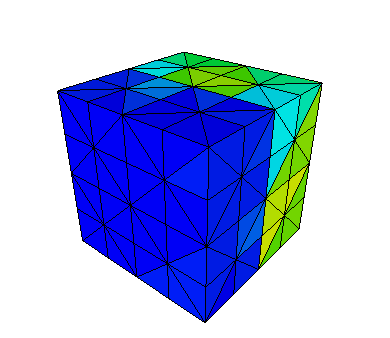
\includegraphics[width=\textwidth]{plots/sigma_it_0_mars.png}}
    \caption{Iter. No. 0.}
\end{subfigure}
	\hfill
\begin{subfigure}[t]{0.49\textwidth}
	\raisebox{-\height}{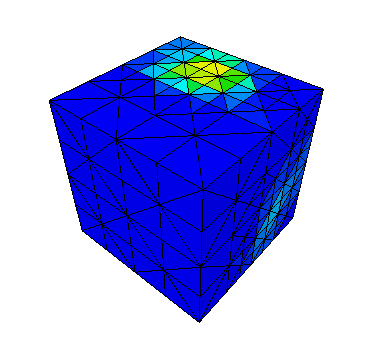
\includegraphics[width=\textwidth]{plots/sigma_it_4_mars.png}}
    \caption{Iter. No. 4.}
\end{subfigure}

\begin{subfigure}[t]{0.49\textwidth}
	\raisebox{-\height}{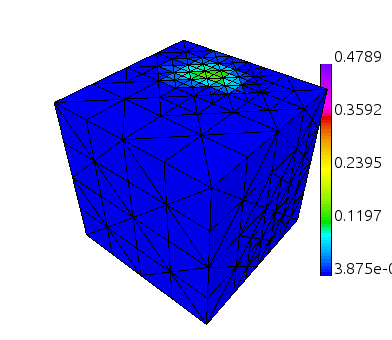
\includegraphics[width=\textwidth]{plots/sigma_it_6_mars.png}}
    \caption{Iter. No. 6.}
\end{subfigure}
	\hfill
\begin{subfigure}[t]{0.49\textwidth}
	\raisebox{-\height}{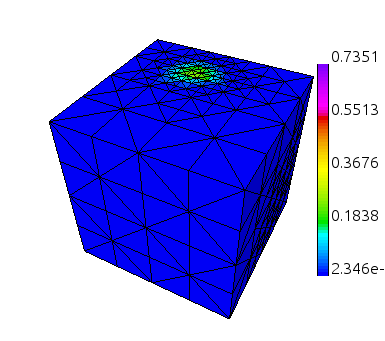
\includegraphics[width=\textwidth]{plots/sigma_it_8_mars.png}}
    \caption{Iter. No. 8.}
\end{subfigure}

\begin{subfigure}[t]{0.49\textwidth}
	\raisebox{-\height}{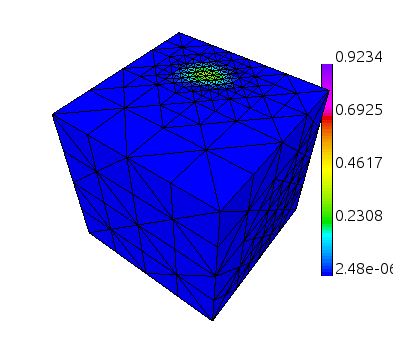
\includegraphics[width=\textwidth]{plots/sigma_it_10_mars.png}}
    \caption{Iter. No. 10.}
\end{subfigure}
	\hfill
\begin{subfigure}[t]{0.49\textwidth}
	\raisebox{-\height}{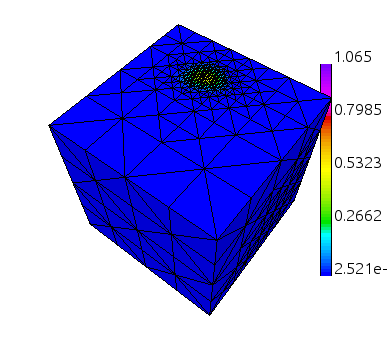
\includegraphics[width=\textwidth]{plots/sigma_it_12_mars.png}}
    \caption{Iter. No. 12.}
\end{subfigure}

\caption{AMR, using MARS refinement in 3D, $\beta = \infty$.}
\label{fig:amr_trans3D_mars}
\end{figure}

\begin{figure}[h!]
\centering
\begin{subfigure}[t]{0.49\textwidth}
	\raisebox{-\height}{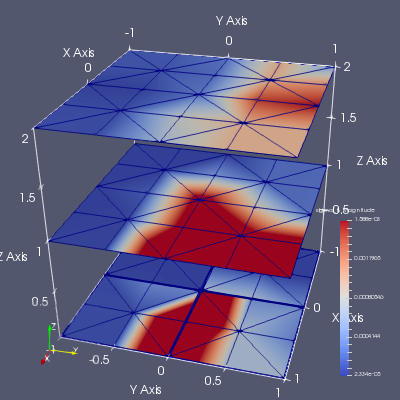
\includegraphics[width=\textwidth]{plots/sigma_mars_pv_it_0.png}}
    \caption{Iter. No. 0.}
\end{subfigure}
	\hfill
\begin{subfigure}[t]{0.49\textwidth}
	\raisebox{-\height}{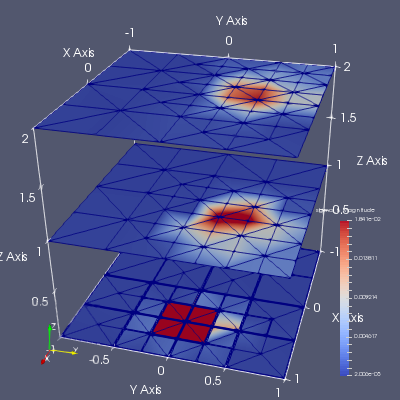
\includegraphics[width=\textwidth]{plots/sigma_mars_pv_it_4.png}}
    \caption{Iter. No. 4.}
\end{subfigure}

\begin{subfigure}[t]{0.49\textwidth}
	\raisebox{-\height}{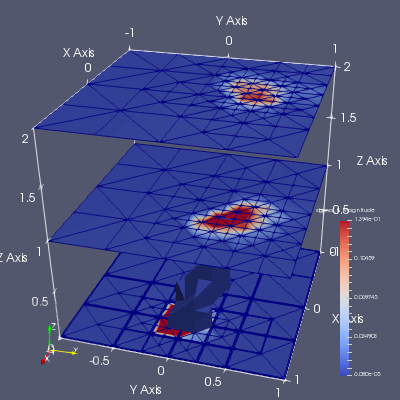
\includegraphics[width=\textwidth]{plots/sigma_mars_pv_it_6.png}}
    \caption{Iter. No. 6.}
\end{subfigure}
	\hfill
\begin{subfigure}[t]{0.49\textwidth}
	\raisebox{-\height}{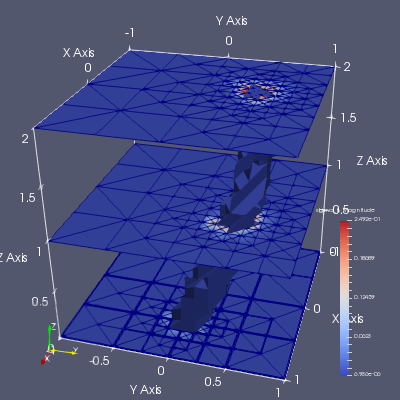
\includegraphics[width=\textwidth]{plots/sigma_mars_pv_it_8.png}}
    \caption{Iter. No. 8.}
\end{subfigure}

\begin{subfigure}[t]{0.49\textwidth}
	\raisebox{-\height}{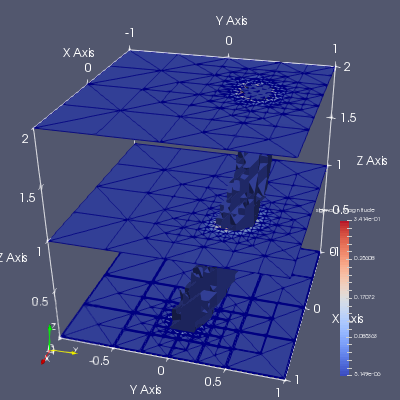
\includegraphics[width=\textwidth]{plots/sigma_mars_pv_it_10.png}}
    \caption{Iter. No. 10.}
\end{subfigure}
	\hfill
\begin{subfigure}[t]{0.49\textwidth}
	\raisebox{-\height}{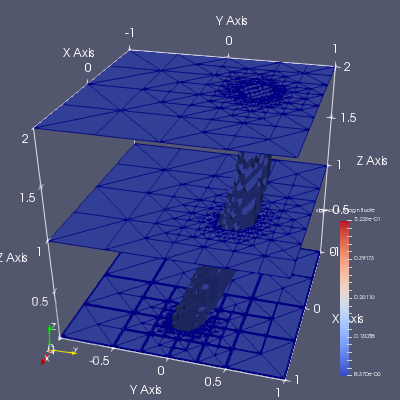
\includegraphics[width=\textwidth]{plots/sigma_mars_pv_it_12.png}}
    \caption{Iter. No. 12.}
\end{subfigure}

\caption{AMR, using MARS refinement in 3D, $\beta = \infty$.}
%pictures generated by ParaView scripts
\label{fig:amr_trans3D_paraview_mars}
\end{figure}

\begin{figure}[h!]
\centering
\begin{subfigure}[t]{0.49\textwidth}
	\raisebox{-\height}{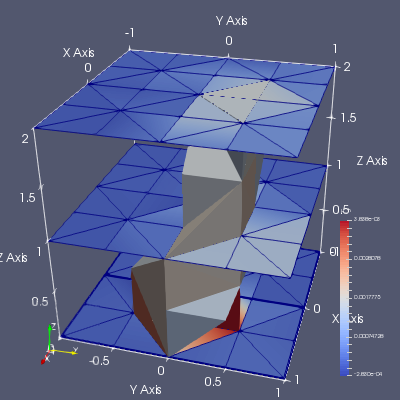
\includegraphics[width=\textwidth]{plots/longruns/u_mfem_it_0.png}}
    \caption{Iter. No. 0.}
\end{subfigure}
	\hfill
\begin{subfigure}[t]{0.49\textwidth}
	\raisebox{-\height}{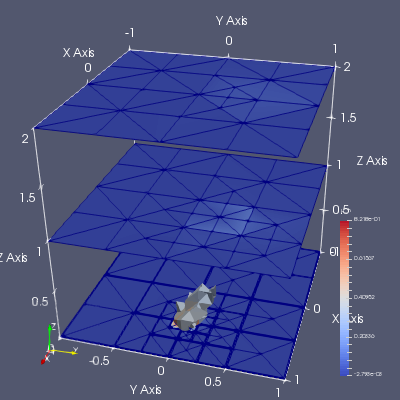
\includegraphics[width=\textwidth]{plots/longruns/u_mfem_it_10.png}}
    \caption{Iter. No. 10.}
\end{subfigure}

\begin{subfigure}[t]{0.49\textwidth}
	\raisebox{-\height}{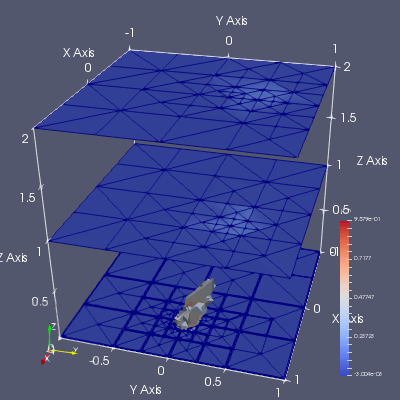
\includegraphics[width=\textwidth]{plots/longruns/u_mfem_it_20.png}}
    \caption{Iter. No. 20.}
\end{subfigure}
	\hfill
\begin{subfigure}[t]{0.49\textwidth}
	\raisebox{-\height}{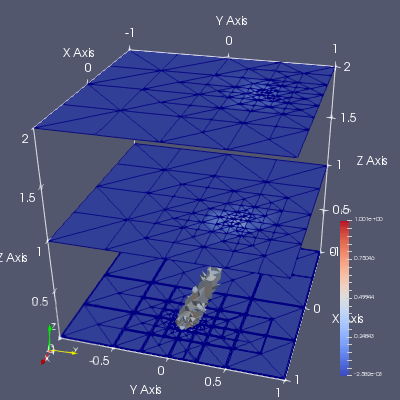
\includegraphics[width=\textwidth]{plots/longruns/u_mfem_it_30.png}}
    \caption{Iter. No. 30.}
\end{subfigure}

\begin{subfigure}[t]{0.49\textwidth}
	\raisebox{-\height}{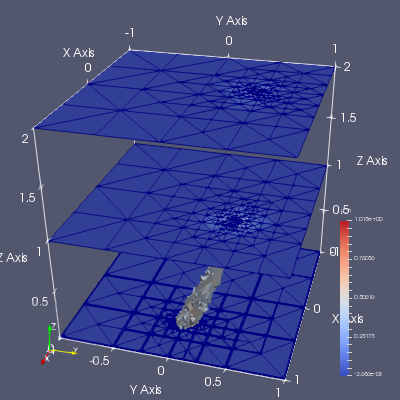
\includegraphics[width=\textwidth]{plots/longruns/u_mfem_it_40.png}}
    \caption{Iter. No. 40.}
\end{subfigure}
	\hfill
\begin{subfigure}[t]{0.49\textwidth}
	\raisebox{-\height}{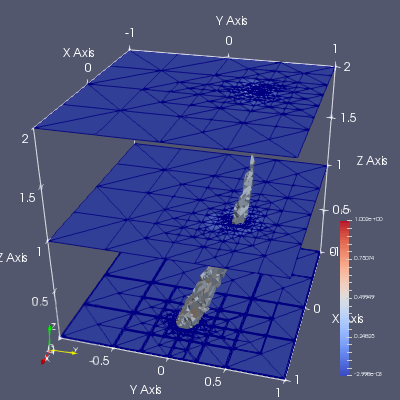
\includegraphics[width=\textwidth]{plots/longruns/u_mfem_it_50.png}}
    \caption{Iter. No. 50.}
\end{subfigure}

\caption{AMR, using MFEM refinement in 3D, $\beta = \infty$, long, part 1.}
%pictures generated by ParaView scripts
%nprocs = 100
\label{fig:amr_trans3D_paraview_mfem_longrun_part1}
\end{figure}

\begin{figure}[h!]
\centering
\begin{subfigure}[t]{0.49\textwidth}
	\raisebox{-\height}{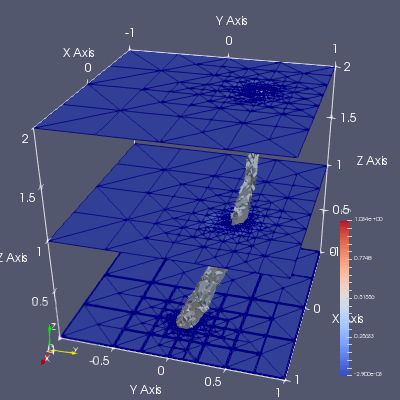
\includegraphics[width=\textwidth]{plots/longruns/u_mfem_it_60.png}}
    \caption{Iter. No. 60.}
\end{subfigure}
	\hfill
\begin{subfigure}[t]{0.49\textwidth}
	\raisebox{-\height}{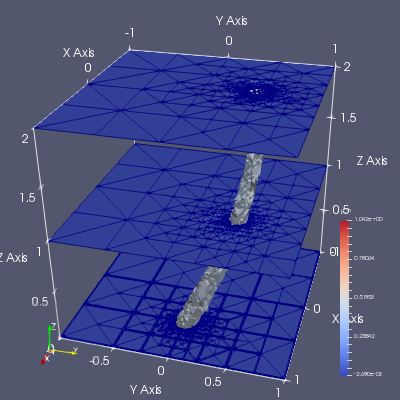
\includegraphics[width=\textwidth]{plots/longruns/u_mfem_it_70.png}}
    \caption{Iter. No. 70.}
\end{subfigure}

\begin{subfigure}[t]{0.49\textwidth}
	\raisebox{-\height}{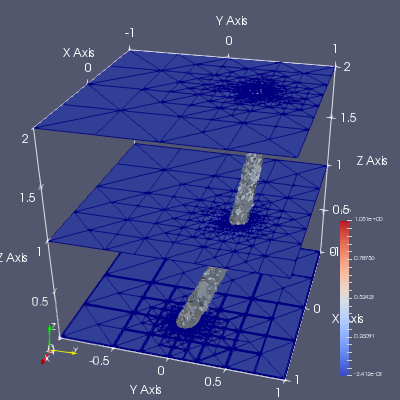
\includegraphics[width=\textwidth]{plots/longruns/u_mfem_it_80.png}}
    \caption{Iter. No. 80.}
\end{subfigure}
	\hfill
\begin{subfigure}[t]{0.49\textwidth}
	\raisebox{-\height}{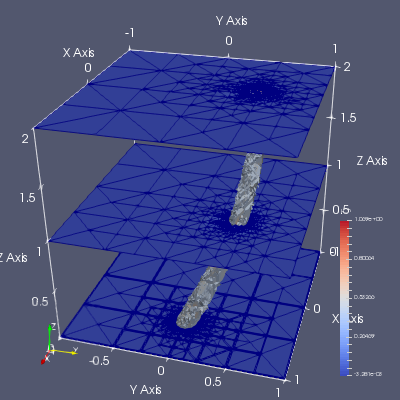
\includegraphics[width=\textwidth]{plots/longruns/u_mfem_it_90.png}}
    \caption{Iter. No. 90.}
\end{subfigure}

\begin{subfigure}[t]{0.49\textwidth}
	\raisebox{-\height}{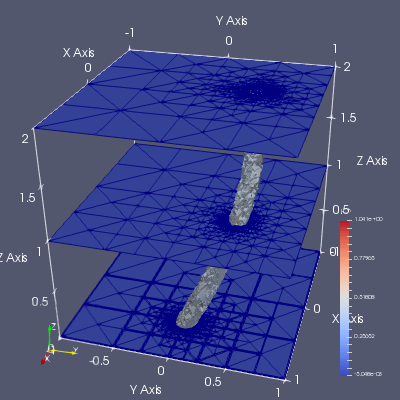
\includegraphics[width=\textwidth]{plots/longruns/u_mfem_it_100.png}}
    \caption{Iter. No. 100.}
\end{subfigure}
	\hfill
\begin{subfigure}[t]{0.49\textwidth}
	\raisebox{-\height}{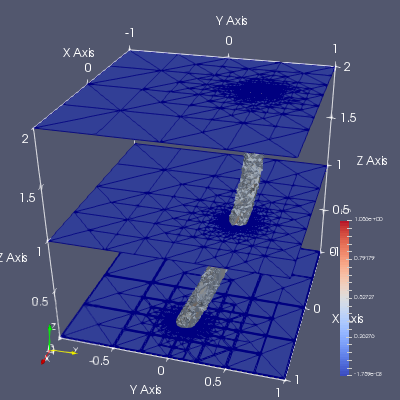
\includegraphics[width=\textwidth]{plots/longruns/u_mfem_it_110.png}}
    \caption{Iter. No. 110.}
\end{subfigure}

\caption{AMR, using MFEM refinement in 3D, $\beta = \infty$, long, part 2.}
%pictures generated by ParaView scripts
%nprocs = 100
\label{fig:amr_trans3D_paraview_mfem_longrun_part2}
\end{figure}

\begin{figure}[h!]
\centering
\begin{subfigure}[t]{0.49\textwidth}
	\raisebox{-\height}{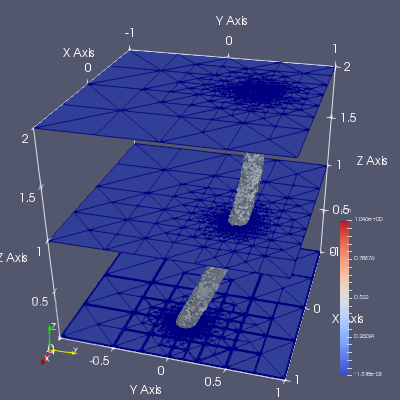
\includegraphics[width=\textwidth]{plots/longruns/u_mfem_it_120.png}}
    \caption{Iter. No. 120.}
\end{subfigure}
	\hfill
\begin{subfigure}[t]{0.49\textwidth}
	\raisebox{-\height}{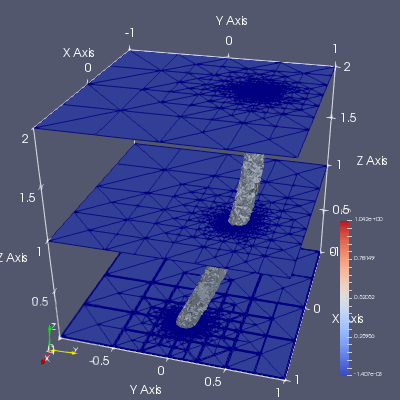
\includegraphics[width=\textwidth]{plots/longruns/u_mfem_it_128.png}}
    \caption{Iter. No. 128.}
\end{subfigure}

\caption{AMR, using MFEM refinement in 3D, $\beta = \infty$, long, part 3.}
%pictures generated by ParaView scripts
%./pvpython /home/kvoronin/Documents/PSU\ project/adaptive\ refinement/paraview_draw.py /home/kvoronin/Downloads/temp/u_mfem_it_ --type 0 --step 10 --stcnt 128 --iso-bot 0.4 --iso-top 1.0 --iso-relative --nsteps 65 --parallel --nprocs 100
%nprocs = 100
\label{fig:amr_trans3D_paraview_mfem_longrun_part3}
\end{figure}

\begin{figure}[h!]
\centering
\begin{subfigure}[t]{0.49\textwidth}
	\raisebox{-\height}{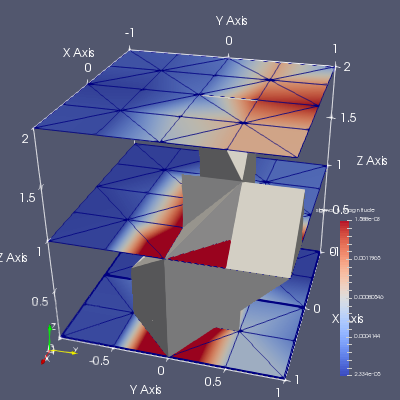
\includegraphics[width=\textwidth]{plots/longruns/sigma_mars_it_0.png}}
    \caption{Iter. No. 0.}
\end{subfigure}
	\hfill
\begin{subfigure}[t]{0.49\textwidth}
	\raisebox{-\height}{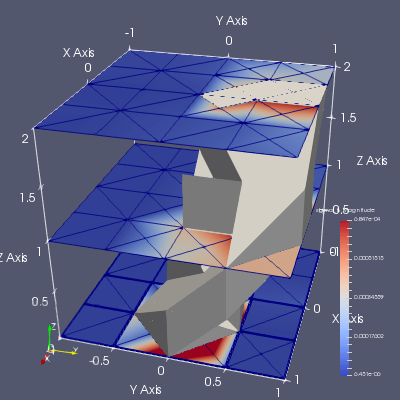
\includegraphics[width=\textwidth]{plots/longruns/sigma_mars_it_2.png}}
    \caption{Iter. No. 2.}
\end{subfigure}

\begin{subfigure}[t]{0.49\textwidth}
	\raisebox{-\height}{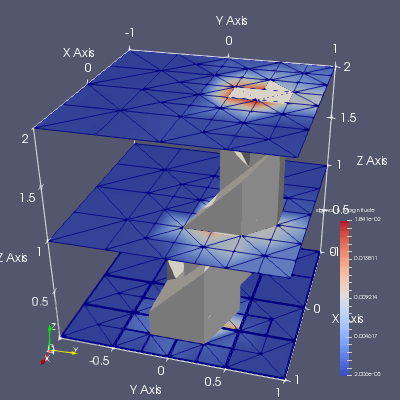
\includegraphics[width=\textwidth]{plots/longruns/sigma_mars_it_4.png}}
    \caption{Iter. No. 4.}
\end{subfigure}
	\hfill
\begin{subfigure}[t]{0.49\textwidth}
	\raisebox{-\height}{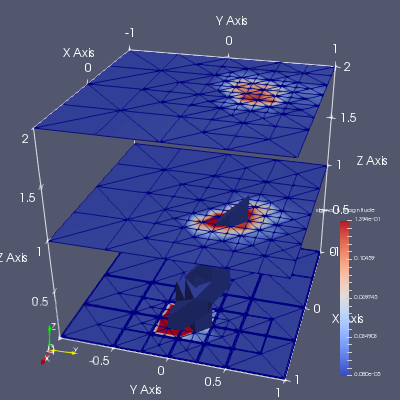
\includegraphics[width=\textwidth]{plots/longruns/sigma_mars_it_6.png}}
    \caption{Iter. No. 6.}
\end{subfigure}

\begin{subfigure}[t]{0.49\textwidth}
	\raisebox{-\height}{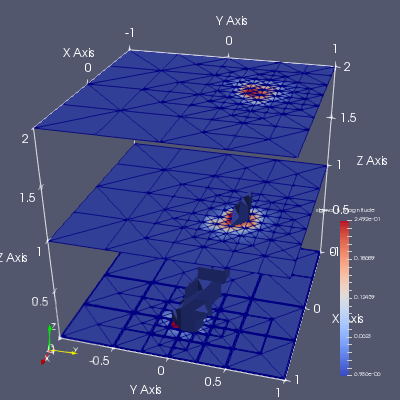
\includegraphics[width=\textwidth]{plots/longruns/sigma_mars_it_8.png}}
    \caption{Iter. No. 8.}
\end{subfigure}
	\hfill
\begin{subfigure}[t]{0.49\textwidth}
	\raisebox{-\height}{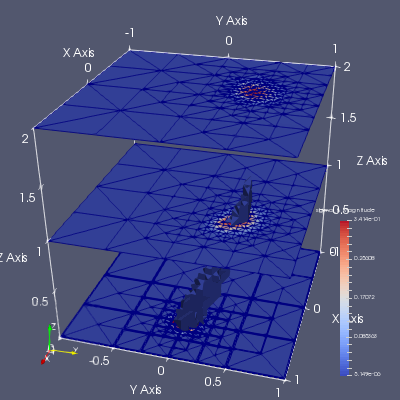
\includegraphics[width=\textwidth]{plots/longruns/sigma_mars_it_10.png}}
    \caption{Iter. No. 10.}
\end{subfigure}

\caption{AMR, using MARS refinement in 3D, $\beta = \infty$, long, part 1.}
%pictures generated by ParaView scripts
%./pvpython /home/kvoronin/Documents/PSU\ project/adaptive\ refinement/paraview_draw.py /home/kvoronin/Downloads/temp/sigma_mars_it_ --type 1 --step 2 --start-count 0 --iso-bot 0.4 --iso-top 1.0 --iso-relative --nsteps 10
\label{fig:amr_trans3D_paraview_mars_longrun_part1}
\end{figure}

\begin{figure}[h!]
\centering
\begin{subfigure}[t]{0.49\textwidth}
	\raisebox{-\height}{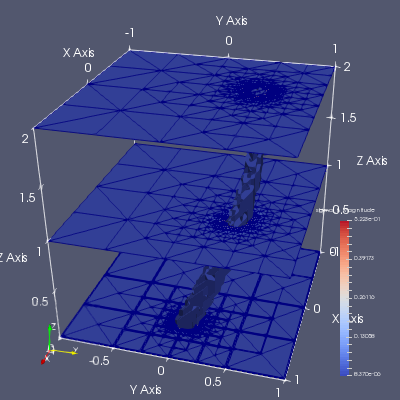
\includegraphics[width=\textwidth]{plots/longruns/sigma_mars_it_12.png}}
    \caption{Iter. No. 12.}
\end{subfigure}
	\hfill
\begin{subfigure}[t]{0.49\textwidth}
	\raisebox{-\height}{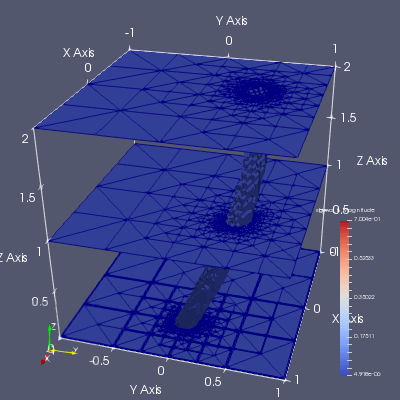
\includegraphics[width=\textwidth]{plots/longruns/sigma_mars_it_14.png}}
    \caption{Iter. No. 14.}
\end{subfigure}

\begin{subfigure}[t]{0.49\textwidth}
	\raisebox{-\height}{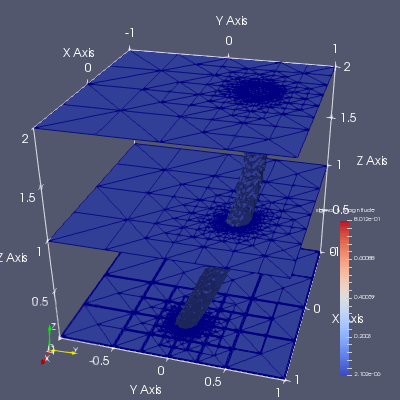
\includegraphics[width=\textwidth]{plots/longruns/sigma_mars_it_16.png}}
    \caption{Iter. No. 16.}
\end{subfigure}
	\hfill
\begin{subfigure}[t]{0.49\textwidth}
	\raisebox{-\height}{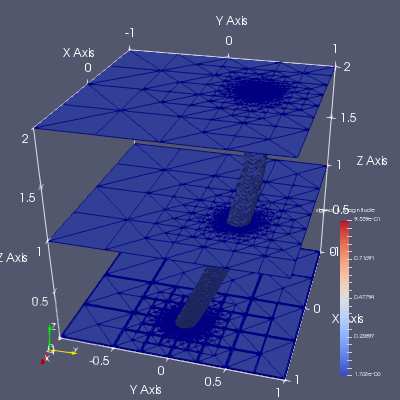
\includegraphics[width=\textwidth]{plots/longruns/sigma_mars_it_18.png}}
    \caption{Iter. No. 18.}
\end{subfigure}

\begin{subfigure}[t]{0.49\textwidth}
	\raisebox{-\height}{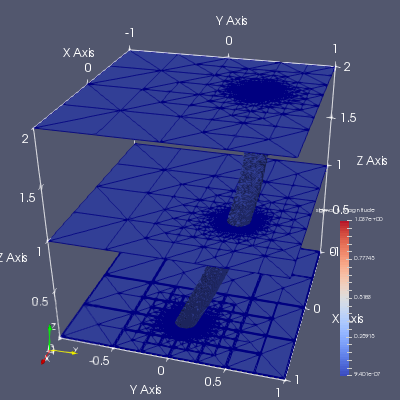
\includegraphics[width=\textwidth]{plots/longruns/sigma_mars_it_20.png}}
    \caption{Iter. No. 20.}
\end{subfigure}

\caption{AMR, using MARS refinement in 3D, $\beta = \infty$, long, part 2.}
%pictures generated by ParaView scripts
%./pvpython /home/kvoronin/Documents/PSU\ project/adaptive\ refinement/paraview_draw.py /home/kvoronin/Downloads/temp/sigma_mars_it_ --type 1 --step 2 --start-count 0 --iso-bot 0.4 --iso-top 1.0 --iso-relative --nsteps 10
\label{fig:amr_trans3D_paraview_mars_longrun_part2}
\end{figure}

\begin{figure}[h!]
\centering
\begin{subfigure}[t]{0.49\textwidth}
	\raisebox{-\height}{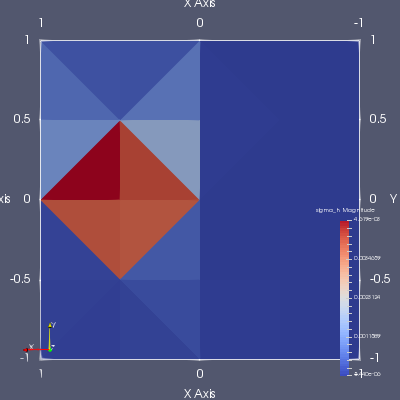
\includegraphics[width=\textwidth]{plots/longruns/sigma_mars_bot_it_0.png}}
    \caption{Iter. No. 0, bot.}
\end{subfigure}
	\hfill
\begin{subfigure}[t]{0.49\textwidth}
	\raisebox{-\height}{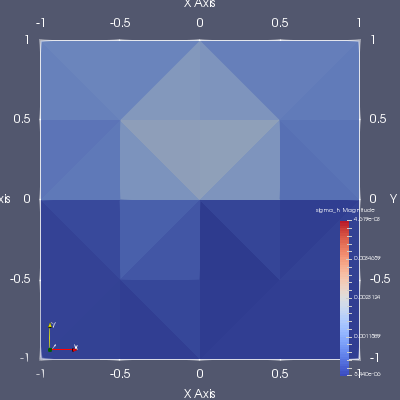
\includegraphics[width=\textwidth]{plots/longruns/sigma_mars_top_it_0.png}}
    \caption{Iter. No. 0, top.}
\end{subfigure}

\begin{subfigure}[t]{0.49\textwidth}
	\raisebox{-\height}{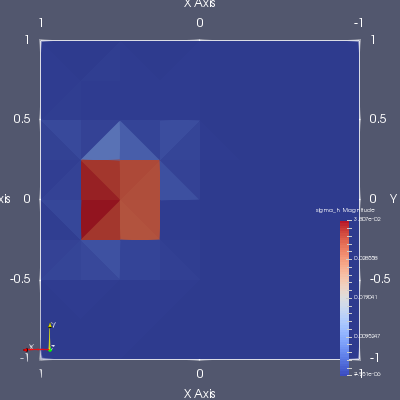
\includegraphics[width=\textwidth]{plots/longruns/sigma_mars_bot_it_4.png}}
    \caption{Iter. No. 4, bot.}
\end{subfigure}
	\hfill
\begin{subfigure}[t]{0.49\textwidth}
	\raisebox{-\height}{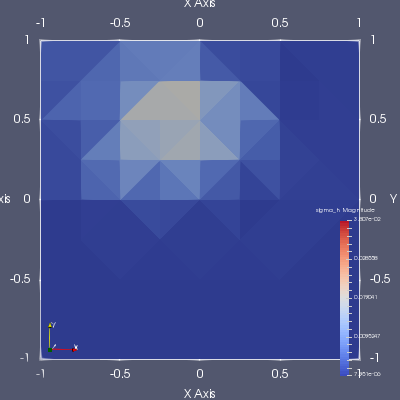
\includegraphics[width=\textwidth]{plots/longruns/sigma_mars_top_it_4.png}}
    \caption{Iter. No. 4, top.}
\end{subfigure}

\begin{subfigure}[t]{0.49\textwidth}
	\raisebox{-\height}{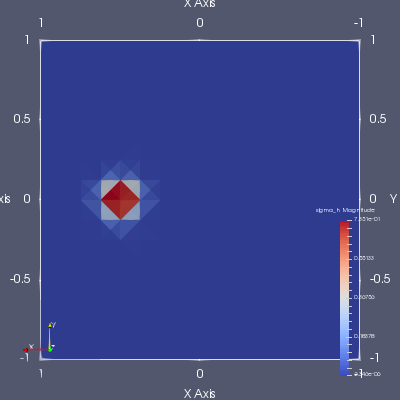
\includegraphics[width=\textwidth]{plots/longruns/sigma_mars_bot_it_8.png}}
    \caption{Iter. No. 8, bot.}
\end{subfigure}
	\hfill
\begin{subfigure}[t]{0.49\textwidth}
	\raisebox{-\height}{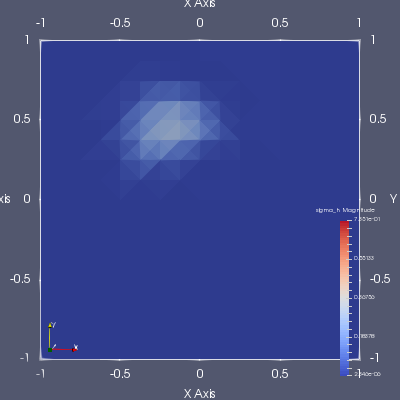
\includegraphics[width=\textwidth]{plots/longruns/sigma_mars_top_it_8.png}}
    \caption{Iter. No. 8, top.}
\end{subfigure}

\caption{AMR, smearing, using MARS refinement in 3D, part 1.}
%pictures generated by ParaView scripts
\label{fig:amr_trans3D_pv_mars_topbot_part1}
\end{figure}

\begin{figure}[h!]
\centering
\begin{subfigure}[t]{0.49\textwidth}
	\raisebox{-\height}{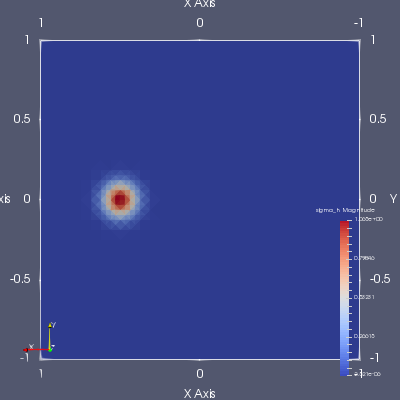
\includegraphics[width=\textwidth]{plots/longruns/sigma_mars_bot_it_12.png}}
    \caption{Iter. No. 12, bot.}
\end{subfigure}
	\hfill
\begin{subfigure}[t]{0.49\textwidth}
	\raisebox{-\height}{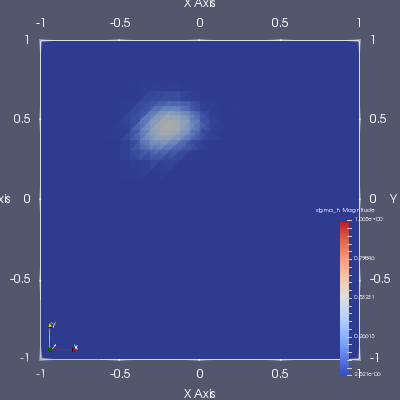
\includegraphics[width=\textwidth]{plots/longruns/sigma_mars_top_it_12.png}}
    \caption{Iter. No. 12, top.}
\end{subfigure}

\begin{subfigure}[t]{0.49\textwidth}
	\raisebox{-\height}{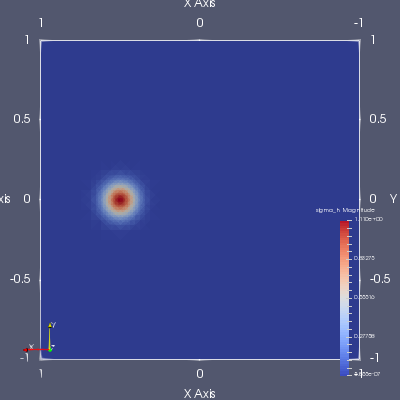
\includegraphics[width=\textwidth]{plots/longruns/sigma_mars_bot_it_16.png}}
    \caption{Iter. No. 16, bot.}
\end{subfigure}
	\hfill
\begin{subfigure}[t]{0.49\textwidth}
	\raisebox{-\height}{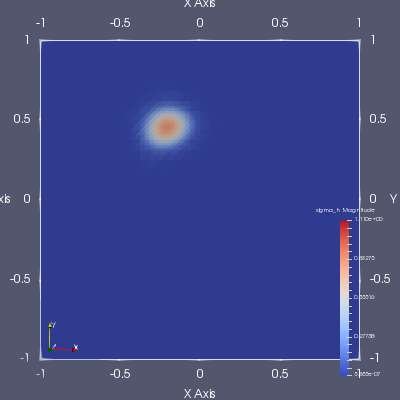
\includegraphics[width=\textwidth]{plots/longruns/sigma_mars_top_it_16.png}}
    \caption{Iter. No. 16, top.}
\end{subfigure}

\begin{subfigure}[t]{0.49\textwidth}
	\raisebox{-\height}{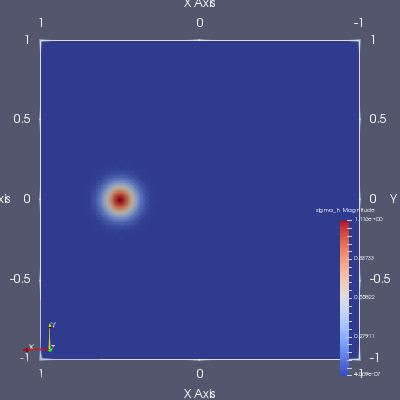
\includegraphics[width=\textwidth]{plots/longruns/sigma_mars_bot_it_18.png}}
    \caption{Iter. No. 18, bot.}
\end{subfigure}
	\hfill
\begin{subfigure}[t]{0.49\textwidth}
	\raisebox{-\height}{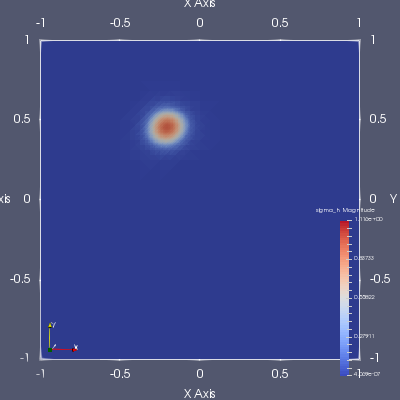
\includegraphics[width=\textwidth]{plots/longruns/sigma_mars_top_it_18.png}}
    \caption{Iter. No. 18, top.}
\end{subfigure}

\caption{AMR, smearing, using MARS refinement in 3D, part 2.}
%pictures generated by ParaView scripts
%visualized as a surface and a bottom or top camera viewpoint
\label{fig:amr_trans3D_pv_mars_topbot_part2}
\end{figure}

\begin{figure}[h!]
\centering
\begin{subfigure}[t]{0.49\textwidth}
	\raisebox{-\height}{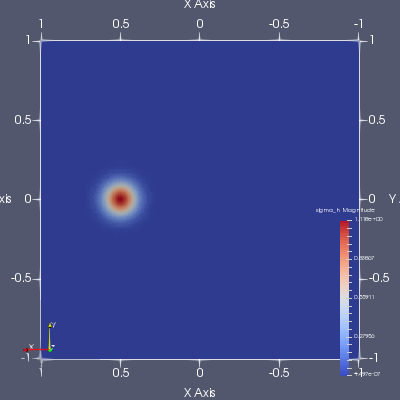
\includegraphics[width=\textwidth]{plots/longruns/sigma_mars_bot_it_20.png}}
    \caption{Iter. No. 20, bot.}
\end{subfigure}
	\hfill
\begin{subfigure}[t]{0.49\textwidth}
	\raisebox{-\height}{\includegraphics[width=\textwidth]{plots/longruns/sigma_mars_top_it_20.png}}
    \caption{Iter. No. 20, top.}
\end{subfigure}

\caption{AMR, smearing, using MARS refinement in 3D, part 3.}
%pictures generated by ParaView scripts
% visualized as slices in paraview
\label{fig:amr_trans3D_pv_mars_topbot_part3}
\end{figure}

\begin{figure}[h!]
\centering
\begin{subfigure}[t]{0.23\textwidth}
	\raisebox{-\height}{\includegraphics[width=\textwidth]{plots/longruns/sigma_it_0_slices_3d_moment_0.png}}
    \caption{Iter. No. 0, $t_0$.}
\end{subfigure}
	\hfill
\begin{subfigure}[t]{0.23\textwidth}
	\raisebox{-\height}{\includegraphics[width=\textwidth]{plots/longruns/sigma_it_0_slices_3d_moment_1.png}}
    \caption{Iter. No. 0, $t_1$.}
\end{subfigure}
	\hfill
\begin{subfigure}[t]{0.23\textwidth}
	\raisebox{-\height}{\includegraphics[width=\textwidth]{plots/longruns/sigma_it_0_slices_3d_moment_2.png}}
    \caption{Iter. No. 0, $t_2$.}
\end{subfigure}
	\hfill
\begin{subfigure}[t]{0.23\textwidth}
	\raisebox{-\height}{\includegraphics[width=\textwidth]{plots/longruns/sigma_it_0_slices_3d_moment_3.png}}
    \caption{Iter. No. 0, $t_3$.}
\end{subfigure}
	
\begin{subfigure}[t]{0.23\textwidth}
	\raisebox{-\height}{\includegraphics[width=\textwidth]{plots/longruns/sigma_it_2_slices_3d_moment_0.png}}
    \caption{Iter. No. 2, $t_0$.}
\end{subfigure}
	\hfill
\begin{subfigure}[t]{0.23\textwidth}
	\raisebox{-\height}{\includegraphics[width=\textwidth]{plots/longruns/sigma_it_2_slices_3d_moment_1.png}}
    \caption{Iter. No. 2, $t_1$.}
\end{subfigure}
	\hfill
\begin{subfigure}[t]{0.23\textwidth}
	\raisebox{-\height}{\includegraphics[width=\textwidth]{plots/longruns/sigma_it_2_slices_3d_moment_2.png}}
    \caption{Iter. No. 2, $t_2$.}
\end{subfigure}
	\hfill
\begin{subfigure}[t]{0.23\textwidth}
	\raisebox{-\height}{\includegraphics[width=\textwidth]{plots/longruns/sigma_it_2_slices_3d_moment_3.png}}
    \caption{Iter. No. 2, $t_3$.}
\end{subfigure}

\begin{subfigure}[t]{0.23\textwidth}
	\raisebox{-\height}{\includegraphics[width=\textwidth]{plots/longruns/sigma_it_4_slices_3d_moment_0.png}}
    \caption{Iter. No. 4, $t_0$.}
\end{subfigure}
	\hfill
\begin{subfigure}[t]{0.23\textwidth}
	\raisebox{-\height}{\includegraphics[width=\textwidth]{plots/longruns/sigma_it_4_slices_3d_moment_1.png}}
    \caption{Iter. No. 4, $t_1$.}
\end{subfigure}
	\hfill
\begin{subfigure}[t]{0.23\textwidth}
	\raisebox{-\height}{\includegraphics[width=\textwidth]{plots/longruns/sigma_it_4_slices_3d_moment_2.png}}
    \caption{Iter. No. 4, $t_2$.}
\end{subfigure}
	\hfill
\begin{subfigure}[t]{0.23\textwidth}
	\raisebox{-\height}{\includegraphics[width=\textwidth]{plots/longruns/sigma_it_4_slices_3d_moment_3.png}}
    \caption{Iter. No. 4, $t_3$.}
\end{subfigure}
	
\begin{subfigure}[t]{0.23\textwidth}
	\raisebox{-\height}{\includegraphics[width=\textwidth]{plots/longruns/sigma_it_6_slices_3d_moment_0.png}}
    \caption{Iter. No. 6, $t_0$.}
\end{subfigure}
	\hfill
\begin{subfigure}[t]{0.23\textwidth}
	\raisebox{-\height}{\includegraphics[width=\textwidth]{plots/longruns/sigma_it_6_slices_3d_moment_1.png}}
    \caption{Iter. No. 6, $t_1$.}
\end{subfigure}
	\hfill
\begin{subfigure}[t]{0.23\textwidth}
	\raisebox{-\height}{\includegraphics[width=\textwidth]{plots/longruns/sigma_it_6_slices_3d_moment_2.png}}
    \caption{Iter. No. 6, $t_2$.}
\end{subfigure}
	\hfill
\begin{subfigure}[t]{0.23\textwidth}
	\raisebox{-\height}{\includegraphics[width=\textwidth]{plots/longruns/sigma_it_6_slices_3d_moment_3.png}}
    \caption{Iter. No. 6, $t_3$.}
\end{subfigure}
	
\begin{subfigure}[t]{0.23\textwidth}
	\raisebox{-\height}{\includegraphics[width=\textwidth]{plots/longruns/sigma_it_8_slices_3d_moment_0.png}}
    \caption{Iter. No. 8, $t_0$.}
\end{subfigure}
	\hfill
\begin{subfigure}[t]{0.23\textwidth}
	\raisebox{-\height}{\includegraphics[width=\textwidth]{plots/longruns/sigma_it_8_slices_3d_moment_1.png}}
    \caption{Iter. No. 8, $t_1$.}
\end{subfigure}
	\hfill
\begin{subfigure}[t]{0.23\textwidth}
	\raisebox{-\height}{\includegraphics[width=\textwidth]{plots/longruns/sigma_it_8_slices_3d_moment_2.png}}
    \caption{Iter. No. 8, $t_2$.}
\end{subfigure}
	\hfill
\begin{subfigure}[t]{0.23\textwidth}
	\raisebox{-\height}{\includegraphics[width=\textwidth]{plots/longruns/sigma_it_8_slices_3d_moment_3.png}}
    \caption{Iter. No. 8, $t_3$.}
\end{subfigure}	

\begin{subfigure}[t]{0.23\textwidth}
	\raisebox{-\height}{\includegraphics[width=\textwidth]{plots/longruns/sigma_it_10_slices_3d_moment_0.png}}
    \caption{Iter. No. 10, $t_0$.}
\end{subfigure}
	\hfill
\begin{subfigure}[t]{0.23\textwidth}
	\raisebox{-\height}{\includegraphics[width=\textwidth]{plots/longruns/sigma_it_10_slices_3d_moment_1.png}}
    \caption{Iter. No. 10, $t_1$.}
\end{subfigure}
	\hfill
\begin{subfigure}[t]{0.23\textwidth}
	\raisebox{-\height}{\includegraphics[width=\textwidth]{plots/longruns/sigma_it_10_slices_3d_moment_2.png}}
    \caption{Iter. No. 10, $t_2$.}
\end{subfigure}
	\hfill
\begin{subfigure}[t]{0.23\textwidth}
	\raisebox{-\height}{\includegraphics[width=\textwidth]{plots/longruns/sigma_it_10_slices_3d_moment_3.png}}
    \caption{Iter. No. 10, $t_3$.}
\end{subfigure}


\caption{AMR, using MFEM refinement in 4D, $\beta = \infty$.}
%pictures generated by ParaView scripts
% ./pvpython ~/Documents/PSU\ project/adaptive\ refinement/paraview_draw_sliceprint.py /home/kvoronin/Downloads/temp/sigma_it_10_slices_3d_moment_ --nsteps 4 --type 1 --iso-bot 0.4 --iso-top 1.0 --iso-relative --step 1 
\label{fig:amr_trans4D_paraview_mars_longrun_part1}
\end{figure}

\begin{figure}[h!]
\centering
\begin{subfigure}[t]{0.23\textwidth}
	\raisebox{-\height}{\includegraphics[width=\textwidth]{plots/longruns/sigma_it_0_slices_withslices_3d_moment_0.png}}
    \caption{Iter. No. 0, $t_0$.}
\end{subfigure}
	\hfill
\begin{subfigure}[t]{0.23\textwidth}
	\raisebox{-\height}{\includegraphics[width=\textwidth]{plots/longruns/sigma_it_0_slices_withslices_3d_moment_1.png}}
    \caption{Iter. No. 0, $t_1$.}
\end{subfigure}
	\hfill
\begin{subfigure}[t]{0.23\textwidth}
	\raisebox{-\height}{\includegraphics[width=\textwidth]{plots/longruns/sigma_it_0_slices_withslices_3d_moment_2.png}}
    \caption{Iter. No. 0, $t_2$.}
\end{subfigure}
	\hfill
\begin{subfigure}[t]{0.23\textwidth}
	\raisebox{-\height}{\includegraphics[width=\textwidth]{plots/longruns/sigma_it_0_slices_withslices_3d_moment_3.png}}
    \caption{Iter. No. 0, $t_3$.}
\end{subfigure}
	
\begin{subfigure}[t]{0.23\textwidth}
	\raisebox{-\height}{\includegraphics[width=\textwidth]{plots/longruns/sigma_it_2_slices_withslices_3d_moment_0.png}}
    \caption{Iter. No. 2, $t_0$.}
\end{subfigure}
	\hfill
\begin{subfigure}[t]{0.23\textwidth}
	\raisebox{-\height}{\includegraphics[width=\textwidth]{plots/longruns/sigma_it_2_slices_withslices_3d_moment_1.png}}
    \caption{Iter. No. 2, $t_1$.}
\end{subfigure}
	\hfill
\begin{subfigure}[t]{0.23\textwidth}
	\raisebox{-\height}{\includegraphics[width=\textwidth]{plots/longruns/sigma_it_2_slices_withslices_3d_moment_2.png}}
    \caption{Iter. No. 2, $t_2$.}
\end{subfigure}
	\hfill
\begin{subfigure}[t]{0.23\textwidth}
	\raisebox{-\height}{\includegraphics[width=\textwidth]{plots/longruns/sigma_it_2_slices_withslices_3d_moment_3.png}}
    \caption{Iter. No. 2, $t_3$.}
\end{subfigure}

\begin{subfigure}[t]{0.23\textwidth}
	\raisebox{-\height}{\includegraphics[width=\textwidth]{plots/longruns/sigma_it_4_slices_withslices_3d_moment_0.png}}
    \caption{Iter. No. 4, $t_0$.}
\end{subfigure}
	\hfill
\begin{subfigure}[t]{0.23\textwidth}
	\raisebox{-\height}{\includegraphics[width=\textwidth]{plots/longruns/sigma_it_4_slices_withslices_3d_moment_1.png}}
    \caption{Iter. No. 4, $t_1$.}
\end{subfigure}
	\hfill
\begin{subfigure}[t]{0.23\textwidth}
	\raisebox{-\height}{\includegraphics[width=\textwidth]{plots/longruns/sigma_it_4_slices_withslices_3d_moment_2.png}}
    \caption{Iter. No. 4, $t_2$.}
\end{subfigure}
	\hfill
\begin{subfigure}[t]{0.23\textwidth}
	\raisebox{-\height}{\includegraphics[width=\textwidth]{plots/longruns/sigma_it_4_slices_withslices_3d_moment_3.png}}
    \caption{Iter. No. 4, $t_3$.}
\end{subfigure}
	
\begin{subfigure}[t]{0.23\textwidth}
	\raisebox{-\height}{\includegraphics[width=\textwidth]{plots/longruns/sigma_it_6_slices_withslices_3d_moment_0.png}}
    \caption{Iter. No. 6, $t_0$.}
\end{subfigure}
	\hfill
\begin{subfigure}[t]{0.23\textwidth}
	\raisebox{-\height}{\includegraphics[width=\textwidth]{plots/longruns/sigma_it_6_slices_withslices_3d_moment_1.png}}
    \caption{Iter. No. 6, $t_1$.}
\end{subfigure}
	\hfill
\begin{subfigure}[t]{0.23\textwidth}
	\raisebox{-\height}{\includegraphics[width=\textwidth]{plots/longruns/sigma_it_6_slices_withslices_3d_moment_2.png}}
    \caption{Iter. No. 6, $t_2$.}
\end{subfigure}
	\hfill
\begin{subfigure}[t]{0.23\textwidth}
	\raisebox{-\height}{\includegraphics[width=\textwidth]{plots/longruns/sigma_it_6_slices_withslices_3d_moment_3.png}}
    \caption{Iter. No. 6, $t_3$.}
\end{subfigure}
	
\begin{subfigure}[t]{0.23\textwidth}
	\raisebox{-\height}{\includegraphics[width=\textwidth]{plots/longruns/sigma_it_8_slices_withslices_3d_moment_0.png}}
    \caption{Iter. No. 8, $t_0$.}
\end{subfigure}
	\hfill
\begin{subfigure}[t]{0.23\textwidth}
	\raisebox{-\height}{\includegraphics[width=\textwidth]{plots/longruns/sigma_it_8_slices_withslices_3d_moment_1.png}}
    \caption{Iter. No. 8, $t_1$.}
\end{subfigure}
	\hfill
\begin{subfigure}[t]{0.23\textwidth}
	\raisebox{-\height}{\includegraphics[width=\textwidth]{plots/longruns/sigma_it_8_slices_withslices_3d_moment_2.png}}
    \caption{Iter. No. 8, $t_2$.}
\end{subfigure}
	\hfill
\begin{subfigure}[t]{0.23\textwidth}
	\raisebox{-\height}{\includegraphics[width=\textwidth]{plots/longruns/sigma_it_8_slices_withslices_3d_moment_3.png}}
    \caption{Iter. No. 8, $t_3$.}
\end{subfigure}	

\begin{subfigure}[t]{0.23\textwidth}
	\raisebox{-\height}{\includegraphics[width=\textwidth]{plots/longruns/sigma_it_10_slices_withslices_3d_moment_0.png}}
    \caption{Iter. No. 10, $t_0$.}
\end{subfigure}
	\hfill
\begin{subfigure}[t]{0.23\textwidth}
	\raisebox{-\height}{\includegraphics[width=\textwidth]{plots/longruns/sigma_it_10_slices_withslices_3d_moment_1.png}}
    \caption{Iter. No. 10, $t_1$.}
\end{subfigure}
	\hfill
\begin{subfigure}[t]{0.23\textwidth}
	\raisebox{-\height}{\includegraphics[width=\textwidth]{plots/longruns/sigma_it_10_slices_withslices_3d_moment_2.png}}
    \caption{Iter. No. 10, $t_2$.}
\end{subfigure}
	\hfill
\begin{subfigure}[t]{0.23\textwidth}
	\raisebox{-\height}{\includegraphics[width=\textwidth]{plots/longruns/sigma_it_10_slices_withslices_3d_moment_3.png}}
    \caption{Iter. No. 10, $t_3$.}
\end{subfigure}

\caption{AMR, using MFEM refinement in 4D, $\beta = \infty$, with slices.}
%pictures generated by ParaView scripts
% ./pvpython ~/Documents/PSU\ project/adaptive\ refinement/paraview_draw_sliceprint.py /home/kvoronin/Downloads/temp/sigma_it_10_slices_3d_moment_ --nsteps 4 --type 1 --iso-bot 0.4 --iso-top 1.0 --iso-relative --step 1 
\label{fig:amr_trans4D_paraview_mars_longrun_part2}
\end{figure}

Next, in Table \ref{tab:ur_conv_3D_HdivL2tran_feorder1} we study convergence for uniformly refined mesh in case when we use higher-order elements (elements one order higher than before). For higher-order elements we neither compute functional value nor were able to run the minimization solver.
The latter is due to the known limitations on usage higher-order Nedelec elements in MFEM.

\begin{table}[h!]
\caption{Uniform refinement, rotating Gaussian hill, $H(\div)-L^2$ formulation for the transport equation, higher order elements}
\label{tab:ur_conv_3D_HdivL2tran_feorder1}
\scalebox{.85}{
\begin{tabular}{|c||c|c|c|} \hline
\#dofs & \#iter 2 & $\varepsilon_{\bsigma}$ \\ \hline
5280   & 1901  & 0.84 \\ \hline
41088  & 5424  & 0.67 \\ \hline
324096 & 19533 & 0.38 \\ \hline 
\end{tabular}}
\end{table}

Now we show the results of adaptive mesh refinement for higher-order elements.

\begin{table}[h!]
\caption{AMR, rotating Gaussian hill $\mathbb{R}^3$, $H(\div)-L^2$ formulation for the transport equation, higher order}
\label{tab:amr2_conv_3D_HdivL2tran_feorder1}
\scalebox{.85}{
\begin{tabular}{|c||c|c|} \hline
\#dofs & \#iter 2 & $\varepsilon_{\bsigma}$  \\ \hline
41088  & 5424 & 0.67 \\ \hline
43376  & 5499 & 0.63 \\ \hline
45404  & 5548 & 0.6  \\ \hline
48472  & 5598 & 0.55 \\ \hline
52459  & 5786 & 0.51  \\ \hline
61451  & 6222 & 0.42  \\ \hline
64051  & 6191 & 0.41  \\ \hline
68081  & 6262 & 0.36  \\ \hline
81123  & 6397 & 0.28  \\ \hline
91007  & 6535 & 0.26  \\ \hline

98107  & 6642 & 0.26  \\ \hline
117308 & 6975 & 0.22  \\ \hline
130091 & 7105 & 0.19  \\ \hline
151513 & 7257 & 0.17  \\ \hline
175670 & 7574 & 0.13   \\ \hline

187058 & 7585 & 0.12  \\ \hline
209330 & 7799 & 0.11   \\ \hline
222115 & 7652 & 0.11   \\ \hline
262318 & 8066 & 0.1   \\ \hline
\end{tabular}}
% conservative strategy, 0.9
% beta = infty
\end{table}

For Table \ref{tab:amr2_conv_3D_HdivL2tran_feorder1} one can find in Figure \ref{fig:amr_transp_feorder1} numerical solution for certain iterations.

\begin{figure}[h!]
\centering
\begin{subfigure}[t]{0.49\textwidth}
	\raisebox{-\height}{\includegraphics[width=\textwidth]{plots/comparison_laplace_feorder0.png}}
	\caption{Laplace, 0th order, $\varepsilon_{\bsigma}$}
\end{subfigure}
	\hfill
\begin{subfigure}[t]{0.49\textwidth}
	\raisebox{-\height}{\includegraphics[width=\textwidth]{plots/comparison_transport_feorder0.png}}
	\caption{Transport, 0th order, $\varepsilon_{\bsigma}$}
\end{subfigure}

\begin{subfigure}[t]{0.3\textwidth}
	\raisebox{-\height}{\includegraphics[width=\textwidth]{plots/comparison_laplace_feorder1.png}}
	\caption{Laplace, 1st order, $\varepsilon_{\bsigma}$}
\end{subfigure}
	\hfill
\begin{subfigure}[t]{0.3\textwidth}
	\raisebox{-\height}{\includegraphics[width=\textwidth]{plots/comparison_laplace_feorder1_u.png}}
	\caption{Laplace, 1st order, $\varepsilon_{u}$}
\end{subfigure}
	\hfill
\begin{subfigure}[t]{0.3\textwidth}
	\raisebox{-\height}{\includegraphics[width=\textwidth]{plots/comparison_transport_feorder1.png}}
	\caption{Transp., 1st order, $\varepsilon_{\bsigma}$.}
	
\end{subfigure}

\caption{Comparison of convergence rates for uniform and adaptive mesh refinement for the two test problems, different orders of f.e.}
% For these pictures, threshold was 0.9
\label{fig:comparison_ur_amr}
\end{figure}

\begin{figure}[h!]
\centering
\begin{subfigure}[t]{0.49\textwidth}
	\raisebox{-\height}{\includegraphics[width=\textwidth]{plots/1000000.png}}
	\caption{$\beta = \infty$}
\end{subfigure}
	\hfill
\begin{subfigure}[t]{0.49\textwidth}
	\raisebox{-\height}{\includegraphics[width=\textwidth]{plots/{1.0}.png}}
	\caption{$\beta = 1.0$}
\end{subfigure}

\begin{subfigure}[t]{0.49\textwidth}
	\raisebox{-\height}{\includegraphics[width=\textwidth]{plots/{0.1}.png}}
	\caption{$\beta = 0.01$}
\end{subfigure}
	\hfill
\begin{subfigure}[t]{0.49\textwidth}
	\raisebox{-\height}{\includegraphics[width=\textwidth]{plots/{0.01}.png}}
	\caption{$\beta = 0.01$}
\end{subfigure}

\begin{subfigure}[t]{0.49\textwidth}
	\raisebox{-\height}{\includegraphics[width=\textwidth]{plots/{0.001}.png}}
	\caption{$\beta = 0.001$}
\end{subfigure}
	\hfill
\begin{subfigure}[t]{0.49\textwidth}
	\raisebox{-\height}{\includegraphics[width=\textwidth]{plots/{0.0001}.png}}
    \caption{$\beta = 0.0001$}
\end{subfigure}

%\subfigure[$\beta = \infty$]{0.49\textwidth}{\includegraphics[scale=.6]{plots/beta_infinity.png}}
%\hfill
%%\subfigure[Solver time (log-log plot)]{\includegraphics[scale=.08,clip,trim=3.5cm 0 7cm 2cm]{plots/beta_infinity.png}}
%\subfigure[$\beta = 1.0$]{\includegraphics[scale=.6]{plots/{beta_1.0}.png}}

%%\subfigure[$\beta = 0.1$]{\includegraphics[scale=.6]{plots/{beta_0.1}.png}}
%\subfigure[$\beta = 0.01$]{\includegraphics[scale=.6]{plots/{beta_0.01}.png}}
%\hfill
%\subfigure[$\beta = 0.001$]{\includegraphics[scale=.6]{plots/{beta_0.001}.png}}
%
%\subfigure[$\beta = 0.0001$]{\includegraphics[scale=.6]{plots/{beta_0.0001}.png}}
\caption{AMR, iteration \# 20, different values of the smoothing parameter $\beta$.}
\label{fig:amr_lapl_beta3D}
\end{figure}

\begin{figure}[h!]
\centering
\begin{subfigure}[t]{0.35\textwidth}
	\raisebox{-\height}{\includegraphics[width=\textwidth]{plots/feorder0_u_it_0.png}}
	\caption{It. 0, $u_h$}
\end{subfigure}
	\hfill
\begin{subfigure}[t]{0.35\textwidth}
	\raisebox{-\height}{\includegraphics[width=\textwidth]{plots/feorder0_sigma_it_0.png}}
	\caption{It. 0, $\bsigma_h$}
\end{subfigure}

\begin{subfigure}[t]{0.35\textwidth}
	\raisebox{-\height}{\includegraphics[width=\textwidth]{plots/feorder0_u_it_5.png}}
	\caption{It. 5, $u_h$}
\end{subfigure}
	\hfill
\begin{subfigure}[t]{0.35\textwidth}
	\raisebox{-\height}{\includegraphics[width=\textwidth]{plots/feorder0_sigma_it_5.png}}
	\caption{It. 5, $\bsigma_h$}
\end{subfigure}

\begin{subfigure}[t]{0.35\textwidth}
	\raisebox{-\height}{\includegraphics[width=\textwidth]{plots/feorder0_u_it_10.png}}
	\caption{It. 10, $u_h$}
\end{subfigure}
	\hfill
\begin{subfigure}[t]{0.35\textwidth}
	\raisebox{-\height}{\includegraphics[width=\textwidth]{plots/feorder0_sigma_it_10.png}}
	\caption{It. 10, $\bsigma_h$}
\end{subfigure}

\begin{subfigure}[t]{0.35\textwidth}
	\raisebox{-\height}{\includegraphics[width=\textwidth]{plots/feorder0_u_it_15.png}}
	\caption{It. 15, $u_h$}
\end{subfigure}
	\hfill
\begin{subfigure}[t]{0.35\textwidth}
	\raisebox{-\height}{\includegraphics[width=\textwidth]{plots/feorder0_sigma_it_15.png}}
	\caption{It. 15, $\bsigma_h$}
\end{subfigure}

\caption{AMR, transport test, f.e. spaces of order 0.}
% For these pictures, threshold was 0.9
\label{fig:amr_transp_feorder0}
\end{figure}


\begin{figure}[h!]
\centering
\begin{subfigure}[t]{0.35\textwidth}
	\raisebox{-\height}{\includegraphics[width=\textwidth]{plots/feorder1_u_it_0.png}}
	\caption{It. 0, $u_h$}
\end{subfigure}
	\hfill
\begin{subfigure}[t]{0.35\textwidth}
	\raisebox{-\height}{\includegraphics[width=\textwidth]{plots/feorder1_sigma_it_0.png}}
	\caption{It. 0, $\bsigma_h$}
\end{subfigure}

\begin{subfigure}[t]{0.35\textwidth}
	\raisebox{-\height}{\includegraphics[width=\textwidth]{plots/feorder1_u_it_5.png}}
	\caption{It. 5, $u_h$}
\end{subfigure}
	\hfill
\begin{subfigure}[t]{0.35\textwidth}
	\raisebox{-\height}{\includegraphics[width=\textwidth]{plots/feorder1_sigma_it_5.png}}
	\caption{It. 5, $\bsigma_h$}
\end{subfigure}

\begin{subfigure}[t]{0.35\textwidth}
	\raisebox{-\height}{\includegraphics[width=\textwidth]{plots/feorder1_u_it_10.png}}
	\caption{It. 10, $u_h$}
\end{subfigure}
	\hfill
\begin{subfigure}[t]{0.35\textwidth}
	\raisebox{-\height}{\includegraphics[width=\textwidth]{plots/feorder1_sigma_it_10.png}}
	\caption{It. 10, $\bsigma_h$}
\end{subfigure}

\begin{subfigure}[t]{0.35\textwidth}
	\raisebox{-\height}{\includegraphics[width=\textwidth]{plots/feorder1_u_it_15.png}}
	\caption{It. 15, $u_h$}
\end{subfigure}
	\hfill
\begin{subfigure}[t]{0.35\textwidth}
	\raisebox{-\height}{\includegraphics[width=\textwidth]{plots/feorder1_sigma_it_15.png}}
	\caption{It. 15, $\bsigma_h$}
\end{subfigure}

\caption{AMR, transport test, f.e. spaces of order 1.}
% For these pictures, threshold was 0.9
\label{fig:amr_transp_feorder1}
\end{figure}

Comparing Figures \ref{fig:amr_transp_feorder0} and \ref{fig:amr_transp_feorder1} it's easy to notice that for the lowest order elements the quality of the results is much poorer. Although the mesh still gets refined around the volume where the solution is concentrated, the solution is dissipating strongly as the time goes. Hence, for the final time the magnitude has already decreased below 30\% of the magnitude at the bottom. Notice that for the exact solution magnitude remains constant in time since the solution is only rotating in space and no dissipation mechanism is present in the problem.
The higher-order elements (see Fig. \ref{fig:amr_transp_feorder1}) provide much higher accuracy.

\section{Numerical results, 4D}

\begin{itemize}
	\item Laplace test. \newline
	Domain: Fichera corner $[-1,1]^3 \times [0,1] \ [0,1]^3 \times [0,1]$ \newline
	Solution: $u = r_\Xx^q$, where $r_\Xx = \sqrt{x^2 + y^2 + z^2}$ with Sobolev regularity $1.5 + q$.
	
	\item Transport test. \newline
	Domain: \newline
	Solution: \newline
\end{itemize}

In Table \eqref{tab:ur_lapl_fichera4D_HdivH1lapl_smooth} one can find convergence results for the smooth solution ($u \in H^2$) of the Fichera corner problem in 4D.

\begin{table}[h!]
\caption{Uniform refinement, Fichera corner in $\mathbb{R}^4$, $H(\div)-H^1$ formulation for the Laplace equation, $q = 1.0$}
\label{tab:ur_lapl_fichera4D_HdivH1lapl_smooth}
\scalebox{.85}{
\begin{tabular}{|c||c|c|c|} \hline
\#dofs & \#iter 2 & $\varepsilon_{\bsigma}$ & $\varepsilon_u$  \\ \hline
20889   & 106 & 0.161 & 0.055  \\ \hline
318945  & 115 & 0.077 & 0.015  \\ \hline 
4986945 & 118 & 0.038 & 0.004 \\ \hline 
\end{tabular}}
\end{table}

Next, we take a less regular solution ($u \in H^{1.6}$).
\begin{table}[h!]
\caption{Uniform refinement, Fichera corner in $\mathbb{R}^4$, $H(\div)-H^1$ formulation for the Laplace equation, $q = 0.1$}
\label{tab:ur_lapl_fichera4D_HdivH1lapl_rougher}
\scalebox{.85}{
\begin{tabular}{|c||c|c|c|} \hline
\#dofs & \#iter 2 & $\varepsilon_{\bsigma}$ & $\varepsilon_u$  \\ \hline
20889   & 106 & 1.692 & 0.062  \\ \hline
318945  & 115 & 1.024 & 0.023  \\ \hline 
4986945 & 117 & 0.642 & 0.009  \\ \hline 
\end{tabular}}
\end{table}

Now, we consider AMR for the less regular solution:
\begin{table}[h!]
\caption{AMR, Fichera corner in $\mathbb{R}^4$, $H(\div)-H^1$ formulation for the Laplace equation, $q = 0.1$}
\label{tab:amr_lapl_fichera4D_HdivH1lapl_rougher}
\scalebox{.85}{
\begin{tabular}{|c||c|c|c|} \hline
\#dofs & \#iter 2 & $\varepsilon_{\bsigma}$ & $\varepsilon_u$ \\ \hline
20889  & 106 & 1.692 & 0.062  \\ \hline
26329  & 118 & 1.767 & 0.062  \\ \hline 
35622  & 122 & 1.519 & 0.055  \\ \hline 
56220  & 118 & 1.236 & 0.044   \\ \hline 
90640  & 113 & 1.109 & 0.033   \\ \hline 
117596 & 121 & 1.013 & 0.023   \\ \hline 
217764 & 120 & 0.751 & 0.014    \\ \hline 
275936 & 118 & 0.594 & 0.0086  \\ \hline 
409927 & 119 & 0.501 & 0.0058  \\ \hline 
758146 & 122 & 0.418 & 0.0038  \\ \hline 
\end{tabular}}
%error_frac = .90;
%betavalue = 0.1;
%strat = 1;
\end{table}

\begin{table}[h!]
\caption{Uniform refinement, Cylinder over a cube in $\mathbb{R}^4$, $H(\div)-L^2$ formulation for the transport equation}
\label{tab:ur_trans_cyl4D}
\scalebox{.85}{
\begin{tabular}{|c||c|c|} \hline
\#dofs & \#iter 2 & $\varepsilon_{\bsigma}$ \\ \hline
23040    & 522  & 1.02  \\ \hline
318945   & 1183 & 0.95 \\ \hline 
5603328  & 2518 & 0.84 \\ \hline 
88866816 & 3293 & 0.69 \\ \hline %lower tolerance, reltol 1.0e-9, time 20813s, 400 mpi processes
%vim *_3161341.out
\end{tabular}}
\end{table}

\begin{table}[h!]
\caption{AMR, Cylinder over a cube in $\mathbb{R}^4$, $H(\div)-L^2$ formulation for the transport equation}
\label{tab:amr_trans_cyl4D}
\scalebox{.85}{
\begin{tabular}{|c||c|c|} \hline
\#dofs & \#iter 2 & $\varepsilon_{\bsigma}$ \\ \hline
23040  & 522  & 1.02  \\ \hline
33150  & 555  & 0.99  \\ \hline 
73930  & 911  & 0.97  \\ \hline 
167844 & 1190 & 0.93  \\ \hline 
441831 & 1415 & 0.89  \\ \hline 
\end{tabular}}
%error_frac = .95;
%betavalue = 0.1;
%strat = 1;
\end{table}

\begin{table}[h!]
\caption{AMR, Cylinder over a cube in $\mathbb{R}^4$, $H(\div)-L^2$ formulation for the transport equation}
\label{tab:amr_trans_mars_longrun_cyl4D}
\scalebox{.85}{
\begin{tabular}{|c||c|c|} \hline
\#dofs & \#iter 2 & $\varepsilon_{\bsigma}$ \\ \hline
1536   & 96   & 1.00  \\ \hline
1939   & 162  & 1.00  \\ \hline 
6365   & 361  & 1.07  \\ \hline 
18278  & 572  & 0.97  \\ \hline 
54488  & 755  & 0.99  \\ \hline 
158018 & 1098 & 0.95  \\ \hline 
396548 & 1230 & 0.91  \\ \hline 

1046366  & 1434 & 0.80  \\ \hline 
2425486  & 1644 & 0.69  \\ \hline 
5508239  & 1750 & 0.59  \\ \hline 
14123750 & 1869 & 0.49  \\ \hline 
38681500 & 2074 & 0.40  \\ \hline %time 10196.9s
\end{tabular}}
%error_frac = .95;
%betavalue = 0.1;
%strat = 1;
%serial run
\end{table}


In Table \ref{tab:ur_trans_cyl4D_mfem_longrun_cont} results are given for parallel uniform refinement in 4D which followed the last mesh produced by serial AMR (cf. Table \ref{tab:amr_trans_mars_longrun_cyl4D}).
\begin{table}[h!]
\caption{AMR, Cylinder over a cube in $\mathbb{R}^4$, $H(\div)-L^2$ formulation for the transport equation}
\label{tab:ur_trans_cyl4D_mfem_longrun_cont}
\scalebox{.85}{
\begin{tabular}{|c||c|c|} \hline
\#dofs & \#iter 2 & $\varepsilon_{\bsigma}$ \\ \hline
38681500  & 2183  & 0.40  \\ \hline %time 7540.98s
618739552 & 5577  & 0.27  \\ \hline %time 39791.3s
\end{tabular}}
%error_frac = .95;
%-np 200 -ppn 10
\end{table}

\section{Conclusion}


\section{Possible things for the paper}

\begin{itemize}
	\item Minimization solver
	\item AMR scheme for the minimization solver, three approaches
	\item Refinement strategies including beta	
	\item Laplace equation in the L-shaped domain and transport in the cube (pictures, comparison with uniform refinement and comparison between different approaches)
\end{itemize}

What would be the main concept (idea) of the paper?

We can say "we suggest a minimization solver for AMR in the considered CFOSLS setting".

I'd like to say that we can efficiently reuse the previous iterations in terms of the iteration count, but the results don't show it.

\section{To-do list}
\begin{itemize}
	\item Write the draft for theoretical sections
	\item Numerical results: tables
	\item Numerical resuls: pictures
	\item Introduction
\end{itemize}

%%%%%%%%%%%%%%%%%%%%%%%%%%%%%%%%%%%%%%
%%%%%%%%%%%%%%%%%%%%%%%%%%%%%%%%%%%%%%
\begin{thebibliography}{99}
\expandafter\ifx\csname url\endcsname\relax
  \def\url#1{\texttt{#1}}\fi
\expandafter\ifx\csname urlprefix\endcsname\relax\def\urlprefix{URL }\fi

\bibitem[WH]{mixedfem_adapt}
B.I. Wohlmuth and R. H. W. Ronald H. W. Hoppe. A comparison of a posteriori error estimators for mixed finite element discretizations by Raviart-Thomas elements. MATH.COMP, 68:1347–1378, 1999.

\bibitem[BMM]{fosls_adapt}
Local error estimates and adaptive refinement for first-order system least squares (FOSLS), M. Berndt, T. Manteuffel, and S. McCormick, E.T.N.A. 6 (1998), pp. 35-43.

\bibitem[AMMJT]{fosls_adapt2}
Efficiency-based adaptive local refinement for first-order system least-squares formulations, J. Adler, T. Manteuffel, S. McCormick, J. Nolting, J. Ruge, and L. Tang, SIAM J. Sci. Comp. 33 (2011), pp. 1-24. 

\bibitem[AV14]{AdlerVassilevski}
{\sc J.~H. Adler, P.~S. Vassilevski,}
``{\em Error Analysis for Constrained First-Order System Least-Squares Finite-Element Methods,}''
SIAM J. Sci. Comput., 36(3), A1071-A1088, 2014.

\bibitem[NVV]{neumueller_vassilevski_villa}
Martin Neumueller, Panayot S. Vassilevski, and Umberto Villa,
``{\em Space-time CFOSLS methods with AMGe upscaling,}''
Available as Lawrence Livermore National Laboratory Technical Report LLNL-CONF-683318, February 18, 2016.

\bibitem[V08]{MLBFP}
{\sc P.~S. Vassilevski,}
``{\em Multilevel Block--Factorization Preconditioners.} 
Matrix-based Analysis and Algorithms for Solving Finite Element Equations'',
Springer, New York, 2008.

\bibitem[EV98]{evans}
{\sc L.C. Evans,}
 ``{\em Partial Differential Equations,}" Providence: American Mathematical Society, ISBN 0-8218-0772-2. 

\bibitem[GT14]{gatica}
{\sc  G. N. Gatica,} ``{\em A simple introduction to the mixed finite element method: Theory and applications,}'' Springer Briefs in Mathematics. Cham: Springer. MR3157367, 2014.

\bibitem[BFKY12]{hypre}
{\sc A.~Baker, R.~Falgout, T.~Kolev, and U.~Yang,} 
``{\em Scaling hypre's Multigrid Solvers to 100,000 Cores}'',
High Performance Scientific Computing: Algorithms and Applications, Springer,  261-279, 2012.

\bibitem[HY02]{boomerAMG}
{\sc V.~E.~Henson and U. M.~ Yang,} ``{\em Boomer{AMG}: A parallel algebraic multigrid solver and preconditioner}'',
Applied Numerical Mathematics 2002; 41(1):155-177.

\end{thebibliography}

\end{document}
